\documentclass{ieeeaccess}
\usepackage[T1]{fontenc}
\usepackage[utf8]{inputenc}
\usepackage{amsmath,amssymb,booktabs,array,graphicx,cite,microtype}
\usepackage{placeins,float,afterpage}
\usepackage[hidelinks]{hyperref}
\newcommand{\authororcid}[1]{\raisebox{0.6ex}{\href{https://orcid.org/#1}{
\includegraphics[height=0.7em]{figures/orcid-icon.pdf}}}}
\usepackage{etoolbox}
\makeatletter
\input{t1pcr.fd}
\makeatother
\DeclareFontShape{T1}{pcr}{n}{n}{<-> ssub * pcr/m/n}{}
\urlstyle{same}
\hypersetup{pdftitle={Integer Kolmogorov-Arnold Networks for IoT Intrusion Detection},pdfauthor={Oleksandr Kuznetsov; Emanuele Pio De Bernardis; Emanuele Frontoni},pdfsubject={Paper 1 IEEE Access working manuscript v0.15.0}}
\newcommand{\BA}{\operatorname{BA}}
\newcommand{\TNR}{\operatorname{TNR}}
\newcommand{\TPR}{\operatorname{TPR}}
\newcommand{\floor}[1]{\left\lfloor #1\right\rfloor}
\newcommand{\smallnote}[1]{\par\vspace{3pt}{\footnotesize #1\par}}
\graphicspath{{figures/}}
\renewcommand{\dbltopfraction}{0.96}
\renewcommand{\textfraction}{0.04}
\renewcommand{\dblfloatpagefraction}{0.70}
\hyphenation{micro-controller micro-controllers pre-processing}
% The publisher's class and assets are unmodified. Only draft metadata is
% suppressed here: publication date, DOI, volume and year are not yet assigned.
% Reserve space for the class abstract/index bullet; the class aliases both widths.
\newlength{\kanidsabstractwidth}
\setlength{\kanidsabstractwidth}{\dimexpr\titlewidth-10pt\relax}
\let\abstractwidth\kanidsabstractwidth
\makeatletter
\patchcmd{\@maketitle}
  {{\vss\doifont Digital Object Identifier\space\@doi\vss}\vspace*{7.4mm}\par}
  {}{}{\PackageError{kanids}{Could not remove unassigned DOI line}{Review the supplied template.}}
\newcommand{\kanidsdraftfoot}{\hbox to\textwidth{{\footervolfont Working manuscript, version 0.15.0}\hfill{\footerpagefont\thepage}}}
\apptocmd{\ps@titlepage}{\def\@oddfoot{\kanidsdraftfoot}\def\@evenfoot{\kanidsdraftfoot}}{}{}
\apptocmd{\ps@headings}{\def\@oddfoot{\kanidsdraftfoot}\def\@evenfoot{\kanidsdraftfoot}}{}{}
\makeatother
\makeatletter
\patchcmd{\IEEEbiographynophoto}{\vskip 4\baselineskip plus 1fil minus 0\baselineskip}{\vskip 4\baselineskip}{}{\PackageError{kanids}{Could not set biography spacing}{Review the supplied template.}}
\patchcmd{\thebibliography}{\addcontentsline{toc}{section}{\refname}}
  {\phantomsection\addcontentsline{toc}{section}{\refname}}{}
  {\PackageError{kanids}{Could not set bibliography destination}{Review the supplied template.}}
\makeatother
\pagestyle{headings}
\begin{document}
\history{Working manuscript, 16 September 2026.}
\doi{}
\title{Integer Kolmogorov--Arnold Networks for IoT Intrusion Detection: Decision-Agreement Certificates and a Microcontroller Case Study}
\author{\uppercase{Oleksandr Kuznetsov}\authororcid{0000-0003-2331-6326}\authorrefmark{1,2,3,*},
\uppercase{Emanuele Pio De Bernardis}\authororcid{0009-0004-7915-5204}\authorrefmark{1},
\mbox{and \uppercase{Emanuele Frontoni}\authororcid{0000-0002-8893-9244}\authorrefmark{4}}}
\address[1]{Department of Theoretical and Applied Sciences, eCampus University, Via Isimbardi 10, Novedrate (CO), 22060, Italy (e-mails: emanuelepio.debernardis@gmail.com; oleksandr.kuznetsov@uniecampus.it)}
\address[2]{SMARTEST Research Center, eCampus University, Via Isimbardi 10, Novedrate (CO), 22060, Italy}
\address[3]{Department of Intelligent Software Systems and Technologies, School of Computer Science and Artificial Intelligence, V.N. Karazin Kharkiv National University, 4 Svobody Sq., 61022 Kharkiv, Ukraine}
\address[4]{Department of Political Sciences, Communication and International Relations, University of Macerata, Via Crescimbeni, 30/32, 62100 Macerata, Italy (e-mail: emanuele.frontoni@unimc.it)}
\corresp{Corresponding author: Oleksandr Kuznetsov (e-mail: oleksandr.kuznetsov@uniecampus.it).}
\tfootnote{}
\markboth{Kuznetsov et al.: Integer KANs for IoT Intrusion Detection}{Kuznetsov et al.: Integer KANs for IoT Intrusion Detection}
\begin{abstract}
We examine decision preservation and implementation cost when a frozen additive integer Kolmogorov--Arnold network is compiled into a sampled lookup table. Exhaustive enumeration of finite-domain edge functions includes integer rounding; signed error intervals give sufficient agreement certificates relative to the coefficient evaluator. A 20,554-byte table certifies 42,206 of 42,209 prepared test decisions, with empirical agreement on all decisions; the coefficient arrays occupy 254 bytes. A controlled ESP32-C3 experiment separates representation, code placement and parameter placement: with Flash code and DRAM parameters, the LUT is about 1.71 times faster. A separate sustained workload cycles the same 500 source flows used by the hardware comparison and records whole-board USB energy and batch time under one boundary. Coefficient-to-LUT energy estimates decrease from 498 to 92.2~$\mu$J per iteration on Mega 2560 and from 0.987 to 0.859~$\mu$J on ESP32-C3. Instrumented runs report observed static, stack and heap components, without claiming an exact whole-system memory peak. A new endpoint-pair-disjoint floating-model experiment gives additive-KAN balanced accuracy 0.8948 and false-positive rate 20.59\%: its balanced accuracy is lower and its false-positive rate higher than those of the evaluated GAM and MLP baselines. The contribution is an auditable integer-export analysis and physical implementation case study, not architectural or operational superiority.
\end{abstract}
\begin{keywords}
Cross-dataset evaluation, explainability, integer inference, Internet of Things, intrusion detection, Kolmogorov--Arnold networks, lookup tables, microcontrollers.
\end{keywords}
\titlepgskip=-21pt
\maketitle

\section{Introduction}
An intrusion detector intended for a small edge device must satisfy several different requirements. It must distinguish attacks from normal traffic in the evaluated population, remain useful when the observation environment changes, and execute within the device's computational and memory constraints. A high score on a random split of one network dataset establishes only part of this evidence. Likewise, a small parameter array does not establish a small complete firmware image, low peak SRAM use, or low energy per decision.

Kolmogorov--Arnold networks (KANs) represent learned transformations through univariate functions on network edges~\cite{liu2024kan}. Their functions can be evaluated from coefficients or compiled into tables. An additive categorical KAN also exposes a direct decomposition of its output into numerical and categorical contributions. The research question is whether this explicit score structure can be retained in a compact integer evaluator and its export error verified under different memory budgets. A requirement to inspect a separate contribution from every input is different from a requirement to inspect a tree decision path. Both can be useful forms of model inspection; neither establishes that the additive model should replace a more accurate or faster detector. The representation, feature preprocessing, and target processor must be assessed together.

This study asks three questions. What decision-agreement certificate can be computed directly from a frozen integer evaluator and its sampled LUT? What memory--uncertainty trade-off is observed between the fixed table sizes? How do representation and memory placement affect measured inference latency, and what whole-board energy cost is observed under sustained prepared-input execution on AVR and RV32 microcontrollers? Native-feature and cross-dataset experiments place these implementation results in the context of the evaluated classifier pipelines.

The contributions are as follows:
\begin{enumerate}
\item A finite-domain agreement analysis of a frozen additive integer KAN and its sampled LUT. Exact signed edge-error extrema yield sufficient threshold certificates, bounds on changes in fixed-cohort metrics, and a measured relation between table size and unresolved decisions.
\item A physical comparison of five frozen implementations on Mega 2560 and ESP32-C3 using 500 common source observations, followed by a controlled ESP32-C3 factorial experiment that separates representation, code placement and parameter placement. A matched 500-flow sustained-batch study reports time and whole-board USB energy, and a separate instrumented workload reports observed RAM components on both boards.
\item An evidence-linked assessment of exact additive explanations, retrospective cross-dataset stress tests and a new endpoint-pair-disjoint comparison with a cubic B-spline logistic GAM. It distinguishes model quality from compilation agreement and retains explicit limits on input overlap and network generalization.
\end{enumerate}

The classification and deployment experiments serve complementary purposes. The device kernels implement native TON\_IoT models; they are not the harmonized joint-source classifiers. The endpoint-pair-disjoint study fits separate floating models under a frozen protocol; these fits do not replace the deployed weights or the integer certificate. No adaptation, drift-recovery method or new architecture search is introduced. The finalization stage also corrects selection and reporting, compiles fixed representations, and extends the physical evidence.

\section{Related Work and Scope}
KANs use learnable univariate edge functions~\cite{liu2024kan}. Integer quantization is an established deployment technique~\cite{jacob2018integer}, and earlier LUT-KAN and DoS studies compile these functions into table representations~\cite{kuznetsov2026lutkan,kuznetsov2026lutdos}. This study examines how the exact arithmetic of two frozen integer representations can be compared and how their memory placement affects execution on two microcontrollers.

QuantKAN studies branch-aware low-bit training and post-training
quantization, while KANtize evaluates the accuracy and hardware cost of
quantized B-spline and complete-spline tabulation
\cite{fuad2025quantkan,errabii2026kantize}.
Earlier LUT-KAN studies define table representations and examine empirical
accuracy--memory--latency trade-offs
\cite{kuznetsov2026lutkan,kuznetsov2026lutdos}.
Formal bounds on differences between neural networks and their quantized
counterparts also predate this work, for example in QEBVerif
\cite{zhang2023qebverif}.
Here, the additive structure and finite Q12 domain permit direct enumeration
of the exact implementation error for each edge, including integer rounding,
and composition into a certificate for threshold agreement with a frozen
integer reference. We quantify both the decisions certified by this bound
and the unresolved cases, alongside measurements of the same exported
representations on AVR and RV32 microcontrollers. The contribution is a verified deployment study and its reproducible arithmetic and hardware evidence. Summing independent edge intervals is elementary; the value here is their exact computation for the frozen rounding rules and the resulting auditable certificates, not a new general verification theory. KANEL\'{E} maps complete learned univariate functions to FPGA LUTs~\cite{Hoang2025KANELE}; our sampled tables interpolate on MCUs and are checked against an integer coefficient reference. Table~\ref{tab:related-work} identifies these boundaries.

\begin{table*}[t]
\caption{Scope relative to the closest compilation and verification work. The present study adds implementation-specific evidence rather than a general new verification theory.}
\label{tab:related-work}
\centering\scriptsize\setlength{\tabcolsep}{3pt}
\begin{tabular}{p{2.25cm}p{3.35cm}p{3.3cm}p{2.75cm}p{4.85cm}}
\toprule
Work & Starting representation and tabulation & Agreement or quality evidence & Model / application & Hardware placement and energy scope\\
\midrule
CPU LUT-KAN~\cite{kuznetsov2026toolkit} & Spline and edge-function tabulation; segment-wise quantization with interpolation & Empirical approximation error and task-level quality & Synthetic benchmarks; DoS case study & Desktop CPU; NumPy and Numba inference backends.\\
MCU LUT-KAN~\cite{kuznetsov2026esl,kuznetsov2026mculut} & Quantized sampled basis functions; fixed-point interpolation & Approximation error and empirical task-level quality & Basis-function benchmarks; multilayer CICIDS2017 IDS & ESL: Cortex-M3 basis-function benchmarks. JSA: cross-platform benchmarks and physical Mega 2560 / ESP32-C3 IDS. The present study examines agreement with a frozen integer reference.\\
KANEL\'{E}~\cite{Hoang2025KANELE} & Complete learned univariate functions mapped to LUTs & Hardware mapping and empirical prediction quality & MNIST, jet classification, tabular and audio benchmarks & FPGA mapping with quantization/pruning; contrasts with sampled interpolation and integer-reference agreement on the measured MCUs.\\
QuantKAN / KANtize~\cite{fuad2025quantkan,errabii2026kantize} & Low-bit KAN quantization; B-spline and complete-spline tabulation & Quantized accuracy and implementation cost & Quantized KANs & Context for low-bit deployment; different from this frozen evaluator's exhaustive signed-error check.\\
QEBVerif~\cite{zhang2023qebverif} & Neural network and quantized counterpart & Bounds on quantization error & Quantized neural networks & Formal-verification context; additive finite-domain enumeration here exploits the particular exported score.\\
This study & Frozen integer coefficients; sampled LUT with interpolation & Exact signed edge intervals; sufficient threshold-agreement certificates & One additive native TON\_IoT score & Mega 2560 and ESP32-C3; controlled code/parameter placement; matched 500-flow batch time and whole-board USB energy; observed RAM components.\\
\bottomrule
\end{tabular}
\end{table*}


Network dataset heterogeneity is a separate source of difficulty. The TON\_IoT literature documents heterogeneous observations and the need to standardize features and attack types~\cite{moustafa2021networkton,alsaedi2020ton,booij2022heterogeneity}. BoT-IoT, UNSW-NB15, and CICIoT2023 provide different collection settings and feature conventions~\cite{koroniotis2019botiot,moustafa2015unsw,neto2023ciciot}. The recent BRIDGE preprint also addresses heterogeneous cross-domain IoT botnet evaluation~\cite{bhilwarawala2026bridge}. Harmonization is consequently treated here as an explicit experimental mapping, not as a new general solution to domain shift.

Our earlier study~\cite{debernardis2026lightweight} already reported quantized conventional classifiers and physical Mega/ESP32-C3 deployment. It did not include KANs. Its timing experiment used two distinct input vectors, each repeated 250 times. Our short-kernel experiment uses 500 distinct source flows shared across implementations, with five reset-separated passes. The main energy study cycles those same 500 source flows under a sustained load/call/checksum boundary; an earlier twenty-input pilot is retained separately. Their amortized times are not individual-kernel latencies. This study also evaluates the specific harmonized and joint-source protocols described below. These changes extend the model and input coverage; they do not make the old and new latency numbers directly comparable. Model fits, representations, feature adapters, and timing cohorts differ, so we do not calculate an optimization speedup against that earlier article.

\section{Experimental Design}
\subsection{Tasks, populations, and evidence}
The main detection task is binary, with attack as the positive class. We use attack-class F1 for native-feature reporting and balanced accuracy for cross-domain comparison:
\begin{equation}
\begin{split}
F_1&=\frac{2TP}{2TP+FP+FN},\\
\BA&=\frac{1}{2}\left(\frac{TN}{TN+FP}+\frac{TP}{TP+FN}\right).
\end{split}
\label{eq:metrics}
\end{equation}
The two terms in balanced accuracy are normal recall $\TNR$ and attack recall $\TPR$. Both are necessary under the extreme class prior of BoT-IoT, where attack-oriented metrics alone can conceal poor normal-traffic recognition.

\begin{table}[t]
\caption{Evaluated dataset populations. CIC denotes the retained target subset, not the complete dataset.}
\label{tab:populations}
\centering\footnotesize
\begin{tabular}{lrrr}
\toprule
Population & Normal & Attack & Total\\
\midrule
TON\_IoT & 50,000 & 161,043 & 211,043\\
BoT-IoT & 477 & 3,668,045 & 3,668,522\\
UNSW-NB15 & 93,000 & 164,673 & 257,673\\
CIC target subset & 27,709 & 400,000 & 427,709\\
\bottomrule
\end{tabular}
\end{table}

Table~\ref{tab:populations} specifies the populations used by the saved experiments. TON\_IoT uses \texttt{train\_test\_network.csv}. BoT-IoT uses the four Full5pc files. The official UNSW-NB15 training and testing CSVs are concatenated solely for external evaluation; neither is used to fit the joint models. This is not an experiment on the official UNSW training/testing split. The CIC loader retains all benign observations and samples at most 400,000 attacks without replacement with seed 42. Thus its evaluated class prior is an imposed subset prior.

We distinguish four evidence layers. The historical dataset-scale fits and their run-level metrics are preserved outputs of the original experimental stage; their summaries were recomputed without rerunning those fits. The separately identified endpoint-pair-disjoint study adds new floating fits and saved row-level test predictions. The integer coefficient/LUT calculations and explanation sums were independently recomputed from fixed headers and prepared arrays. Finally, physical measurements were collected on the two boards and checked against archived serial traces and build artifacts. Agreement at one layer is not used to claim independent replication at another.

\subsection{Three feature families}
\label{sec:features}
The native TON\_IoT family selects ten numerical fields from sixteen candidates and retains four native categorical fields. In the deployed additive KAN, the numerical order is \texttt{src\_ip\_bytes}, \texttt{dst\_port}, \texttt{dst\_ip\_bytes}, \texttt{src\_port}, \texttt{duration}, \texttt{src\_bytes}, \texttt{dst\_pkts}, \texttt{dst\_bytes}, \texttt{src\_pkts}, and \texttt{dns\_qtype}. The categorical fields are \texttt{proto}, \texttt{service}, \texttt{conn\_state}, and \texttt{dns\_rejected}, with 4, 10, 14, and 4 entries, respectively, including an unknown-category slot. This native representation includes ports.

The rich harmonized family instead defines thirteen numerical candidates and two mapped categorical fields. Let $d$ be duration, $b_s,b_d$ the directional byte counts, and $p_s,p_d$ the directional packet counts. Set $b=b_s+b_d$ and $p=p_s+p_d$. The thirteen candidates are
\begin{equation}
\begin{split}
\mathcal H=\bigg\{&d,b_s,b_d,p_s,p_d,b,p,\frac{b_s-b_d}{b+1},\frac{p_s-p_d}{p+1},\\[-2pt]
&\frac{b_s}{p_s+1},\frac{b_d}{p_d+1},\frac{p}{d+\epsilon},\frac{b}{d+\epsilon}\bigg\},
\quad \epsilon=10^{-6}.
\end{split}
\label{eq:harmonized}
\end{equation}
TON\_IoT uses IP-level byte counts. The terms $b_s/(p_s+1)$ and $b_d/(p_d+1)$ are smoothed directional byte-per-packet ratios, not physical packet means or payload sizes. Equal formulas do not by themselves establish identical byte-accounting and flow-extraction conventions across datasets. Protocol is mapped to TCP, UDP, ICMP, or other; state is mapped to established, closed, rejected, incomplete, reset, or other. Ports, addresses, application-specific metadata, and BoT window aggregates are excluded. Mutual information (MI) retains ten of the thirteen numerical candidates inside each training fit; the resulting rich model has ten numerical and two categorical inputs.

The reduced family, used for the CIC external evaluation, has six numerical inputs: $d,b,p,b/(p+1),p/(d+\epsilon),b/(d+\epsilon)$, plus protocol and state. CIC duration, packet count, and bytes are mapped from \texttt{flow\_duration}, \texttt{Number}, and \texttt{Tot sum}. State uses flag indicators with reset/closed precedence. This mapping is a proxy: CIC observations and source flow logs do not have identical collection units. Reduced models are separately fitted historical models, not rich models with columns removed after training.

\subsection{Preprocessing and model configurations}
Numerical preprocessing coerces values, imputes zero, ranks candidates by MI on at most 40,000 training rows, and selects the required numerical inputs. Selected skewed fields receive $\log(1+\max(v,0))$. A training-fitted normal-output quantile transform, requesting at most 1,000 quantiles, is clipped to $[-3.5,3.5]$. Its subsampling follows the recorded library version. Category vocabularies are fitted on training values, with index zero reserved for unseen categories. An unknown slot is represented explicitly; its contribution is not assumed to be zero. The MI target depends on the fitting stage. Native cross-validation uses the task label: binary for binary fits and attack type for ten-class fits. The canonical additive and multilayer KAN deployment adapters use the multiclass attack-type target even for binary prediction; the frozen DT5 and MLP16 adapters use the binary target. Harmonized fits use the binary target. Stratification by attack type is distinct from the MI target. The native summaries in Table~\ref{tab:supp-native-cv} are retained historical results, and the release records the corresponding task-dependent code path and corrected metadata; no new cross-validation fit is claimed.

The additive KAN uses degree-eight Chebyshev functions and categorical tables, optimized for 250 full-batch gradient steps with learning rate 0.3 and $L_2$ coefficient $10^{-4}$. The multilayer KAN has sixteen hidden units, degree-eight functions in both layers, categorical contributions to the hidden units, and a $\tanh$ intermediate activation. It uses 300 full-batch Adam steps with learning rate 0.01, $(\beta_1,\beta_2)=(0.9,0.999)$, and $\epsilon=10^{-8}$. Both use inverse-class-frequency weighted binary cross-entropy.

For the auxiliary multiclass results, additive KAN uses 300 full-batch steps and multilayer KAN uses 300 Adam steps, with weighted softmax cross-entropy and the same respective learning rates. Multiclass balanced accuracy denotes the mean recall over ten classes.

The baselines are a depth-five balanced decision tree (DT5), a sixteen-unit MLP with early stopping and a 300-iteration limit, LightGBM with 400 estimators and 31 leaves, and XGBoost with 300 estimators and depth six. Both boosting configurations use learning rate 0.05. The MLP uses one-hot categories; the tree and boosting models receive ordinal category codes. DT5 and LightGBM use balanced class weights, while no class-balancing weights are passed to MLP or XGBoost. These are comparisons of the specified pipelines, not an isolation of architecture under identical weighting and categorical encoding. Exact constructor arguments and software records are retained with the source checkpoint.

The ten-feature deployment budget and the sixteen-unit, degree-eight multilayer configuration are inherited compact configurations, rather than validation optima. Preserved selection records favor sixteen numerical features for native additive-KAN F1 and select 32/6 under the one-standard-error rule, whose retained validation threshold is 0.99617. The validation split depends on the seed and is common to the compared candidates within each seed. The saved five-seed validation BA is 0.996023 for 16/8 and 0.996308 for 32/6. Independent inspection of recovered AVR relocatable objects confirms model-array sizes of 5,244 and 9,452 bytes (+80.2\%). Their saved compiler records report \texttt{main} function frames of 155 and 219 bytes (+41.3\%). These probes use a historical kernel and separately trained weights, rather than the exact measured firmware. The figures therefore describe those probes, not total linked Flash, current firmware stack use or measured peak SRAM. The observed validation difference does not establish equivalence. We retain 16/8 as the lower-memory frozen deployment choice; this does not make it the 1-SE selection or a proved optimum.

\subsection{Splits and joint-source selection}
Native evaluation uses five folds for each of seeds 42, 43, and 44, giving fifteen fits per model. Stratification follows the ten-class label. The separate canonical deployment split uses seed 42, with 168,834 training and 42,209 test rows. Native cross-validation covers the whole dataset; it is not nested inside that canonical training pool, and its observations overlap the canonical holdout.

Rich in-domain evaluation uses five binary-stratified folds for each seed from 42 through 51, giving fifty fits per model. Direct transfer fits each source pool and evaluates the complete target for each of ten seeds. A training-only attack:normal cap of 50:1 leaves TON\_IoT unchanged and reduces the full BoT source fit to 477 normal and 23,850 attack rows. Evaluation populations retain their original class proportions.

Joint training uses an outer 80/20 split independently in each source domain and an inner 80/20 split within each outer training pool. The two domains contribute equal numbers of normal observations and use the same candidate attack:normal ratio from $\{5,10,20,50,100\}$. Selection maximizes validation balanced accuracy averaged across six models, two domains, and ten seeds. Validation retains natural priors. The globally selected normal:attack ratio is 1:5; this same ratio also wins separately in each of the ten seed-level validation summaries. A row that belongs to an outer test under one seed can contribute to validation under another seed. Thus the global selection is not strictly nested with wholly untouched outer tests, although separate per-seed selection would return the same ratio in all ten cases. Each final fit combines 382 normal and 1,910 attack observations per domain, totaling 4,584 rows. Inner selection at ratio five instead uses 3,672 fit rows; selection and final refitting have different sample counts.

All the historical splits above are random at observation level. Those pipelines do not establish host-, session-, or time-disjoint evaluation, or deduplication across splits. The new endpoint-pair-disjoint study in Section~\ref{sec:pair-stage2} is separate and does not retroactively change these splits. Training-only preprocessing limits direct fitting on evaluation values but does not remove these broader dependence risks. In the canonical deployment split, 5,201 of 42,209 test rows (12.322\%) exactly match at least one training row across all 44 original CSV columns, including labels and addresses. Row indices are disjoint, but their observed contents need not be. This quantifies dependence in this split; it neither identifies repeated physical events nor measures the resulting optimism in predictive metrics. Section~\ref{sec:duplicate-sensitivity} reports a frozen-model sensitivity analysis on these two subsets.

\subsection{Historical exposure and interpretation}
An initial joint-ratio decision followed inspection of a test-based grid. A later validation-only selection returned the same ratio; the old grid is retained separately and excluded from current selection evidence. The inherited sampled-LUT setting likewise used test-vector margins before the corrected procedure in Section~\ref{sec:lut}. These corrections specify a reproducible current procedure, but they do not make previously inspected tests untouched. UNSW and CIC are therefore retrospective external stress tests of frozen models. We do not treat them as newly blinded confirmation or tune a new adaptation method against them.

\section{Integer Compilation and Decision Preservation}
\subsection{Additive score and coefficient representation}
Here, \emph{integer KAN} means post-training deployment with quantized parameters and integer inference, not training with integer arithmetic. Both the coefficient evaluator and the sampled LUT are integer implementations. The training model uses floating-point Chebyshev coefficients; export approximates its functions with cubic splines and quantizes them. The subsequent LUT stores signed 16-bit samples of the already fixed integer functions. Thus quantization changes numerical precision, while LUT compilation changes how those functions are evaluated. Sampling and interpolation may introduce further score error, which is bounded separately below.

Let $x_i$ denote a transformed numerical feature and $c_j$ a categorical index. The floating additive model is
\begin{equation}
\begin{split}
z(x,c)&=\sum_{i=1}^{10}\phi_i(x_i)+\sum_{j=1}^{4}\psi_j(c_j),\\
\phi_i(x_i)&=\sum_{d=0}^{8}a_{id}T_d(x_i/3.5),
\end{split}
\label{eq:additive}
\end{equation}
with the Chebyshev argument clipped to $[-1,1]$. Constant components are included in the functions; no separate intercept is required by the summed kernel. The binary decision is $\widehat y=\mathbf 1[z\geq0]$.

Export approximates each fixed learned numerical function with a cubic B-spline using sixteen intervals and nineteen coefficients. The representation fit uses 30,000 training locations and 200 uniform anchors, whose least-squares equations receive a factor of 0.1. This fits a representation to the frozen function, not a new classifier to labels. The coefficients become signed 8-bit integers with per-edge signed 16-bit multipliers. Categories use signed 8-bit tables and four signed 16-bit multipliers.

Prepared numerical inputs are
\begin{equation}
q_i=\operatorname{round}_{\rm even}\!\left(4096\,\frac{\operatorname{clip}(x_i,-3.5,3.5)}{3.5}\right),
\end{equation}
with $q_i\in\{-4096,\ldots,4096\}$. Let $F=32768$, $C_{i,s+r}$ be the four local coefficients, and $b_r(q_i)$ the fixed-point cubic basis numerators, approximating $6F$ times the real-valued basis. The implemented score is
\begin{align}
f_i(q_i)&=\floor{\frac{M_i\sum_{r=0}^{3}b_r(q_i)C_{i,s+r}}{F}},\\
g_j(c_j)&=6M^{\rm cat}_j C^{\rm cat}_{o_j+c_j},\\
Z(q,c)&=\sum_{i=1}^{10}f_i(q_i)+\sum_{j=1}^{4}g_j(c_j).
\label{eq:integer}
\end{align}
The decision is $\mathbf1[Z\geq0]$. Floors reproduce signed arithmetic shifts. $Z$ is an integer score, not a calibrated probability. Appendix~\ref{app:arithmetic} defines the basis arithmetic.

The kernel evaluates the potentially wide multiply-shift exactly through
\begin{equation}
\floor{\frac{am}{F}}=hm+\floor{\frac{\ell m}{F}},\quad
h=\floor{a/F},\quad \ell=a-hF,
\end{equation}
using bounded 32-bit products. Its parameter arrays occupy $190+20+32+8+4=254$ bytes: numerical coefficients, numerical multipliers, category entries, category multipliers, and offsets. This count excludes executable code, framework, test fixtures, and runtime storage.

\subsection{Sampled LUT and selection rule}
\label{sec:lut}
The LUT is constructed from the frozen integer coefficient evaluator. For candidate $L$, use $L$ equally spaced nodes with $\Delta=8192/(L-1)$ and $q_k=-4096+k\Delta$. Each edge has the smallest nonnegative exponent $r_i$ for which
\begin{equation}
T_{ik}=\operatorname{round}_{\rm even}(f_i(q_k)/2^{r_i})
\end{equation}
fits the symmetric signed-16-bit magnitude limit 32,767. For $u=\operatorname{clip}(q+4096,0,8192)$, set $k=\min(\floor{u/\Delta},L-2)$ and $v=u-k\Delta$. Evaluation is
\begin{equation}
\widetilde f_i(q)=2^{r_i}\left[T_{ik}+\floor{\frac{(T_{i,k+1}-T_{ik})v}{\Delta}}\right].
\label{eq:lut}
\end{equation}
Rounding precedes scale restoration. Thus this expression is not replaced by floating interpolation followed by one final rounding. Category terms are unchanged.

All 8,193 admissible integer inputs are enumerated separately for each numerical edge:
\begin{equation}
E_i(L)=\max_q|\widetilde f_i(q)-f_i(q)|,\qquad
B(L)=\sum_{i=1}^{10}E_i(L).
\end{equation}
The triangle inequality gives $|\widetilde Z-Z|\leq B(L)$. Therefore
\begin{equation}
|Z|>B(L)\quad\Longrightarrow\quad
\mathbf1[Z\geq0]=\mathbf1[\widetilde Z\geq0].
\label{eq:certificate}
\end{equation}
The statement assumes valid category codes, identical category terms, the specified arithmetic, and no overflow or undefined signed operations. It certifies representation agreement, not correctness of the class label. Exhaustive per-edge enumeration is sufficient for the bound; the procedure does not enumerate every combination of fourteen input fields.

The fixed candidate grid contains 9, 17, 33, 65, 129, 257, 513, and 1025 nodes. Selection uses only explicitly identified training calibration inputs. It chooses the smallest candidate satisfying $B(L)<\min_{(q,c)\in\mathcal T}|Z(q,c)|$; if none satisfies this condition, it selects the largest grid member. The procedure uses training scores, not labels or test F1. The protocol and selected header are frozen before the separate test-evaluation command.

\begin{table}[t]
\caption{Freshly recomputed LUT selection on 168,834 preserved training inputs. ``Uncertified'' counts rows with $|Z|\leq B$.}
\label{tab:lut}
\centering\footnotesize\setlength{\tabcolsep}{4pt}
\begin{tabular}{rrrrr}
\toprule
$L$ & Parameter bytes & $B(L)$ & Uncertified & Mismatches\\
\midrule
9 & 234 & 16,533,344 & 168,834 & 744\\
17 & 394 & 8,439,408 & 128,577 & 239\\
33 & 714 & 2,897,380 & 22,087 & 73\\
65 & 1,354 & 825,654 & 4,597 & 23\\
129 & 2,634 & 219,538 & 1,418 & 6\\
257 & 5,194 & 56,586 & 374 & 1\\
513 & 10,314 & 14,850 & 95 & 0\\
1025 & 20,554 & 4,271 & 34 & 0\\
\bottomrule
\end{tabular}
\end{table}

The minimum absolute training score is 336. No candidate passes the all-training sufficient condition, so $L=1025$ is selected by the fallback (Table~\ref{tab:lut}). Its error bound is 4,271 integer-score units. It certifies 168,800 of 168,834 training decisions, and all training decisions agree empirically. The $L=513$ candidate also has zero empirical training mismatches. Consequently $L=1025$ is neither a proved optimum nor the smallest empirically lossless table. The fallback completes the corrected fixed-grid selection procedure when its sufficient condition fails. The signed-error analysis below was performed later and is not the criterion that selected this table. The single training mismatch at $L=257$ provides a concrete example: original zero-based CSV row 46,815 has coefficient score 488 and LUT score $-116$, changing attack to normal although its label is attack. The sufficient margin condition does not cover this row. The full test still has zero decision differences at $L=257$; this example is not evidence of a test-$F_1$ decrease.

The selected model arrays occupy $20L+54=20,554$ bytes, or 80.921 times the coefficient arrays. Post-freeze evaluation gives identical decisions on all 42,209 canonical test rows. Four rows fail the sufficient margin condition, although their decisions still agree. The coefficient and LUT confusion counts are $TP=31,313$, $FP=214$, $FN=896$, and $TN=9,786$, yielding $F_1=0.9825844$. These are independently recomputed host integer-model results on preserved transformed arrays, not a physical replay of the whole test set. Earlier test exposure remains disclosed as specified above.

\begin{table}[t]
\centering\footnotesize\setlength{\tabcolsep}{3pt}
\caption{Signed-error certificate at threshold zero. The extrema are exact on the Cartesian Q12 domain; $U_{tr}$ and $U_{te}$ count decisions left uncertified on the fixed training and test inputs. All empirical decision differences are zero. This retrospective analysis does not alter selection.}
\label{tab:signed_certificate}
\begin{tabular}{rrrrrr}
\toprule
$L$ & Bytes & $D_-$ & $D_+$ & $U_{tr}$ & $U_{te}$\\
\midrule
513 & 10,314 & $-10065$ & 8250 & 64 & 12\\
1025 & 20,554 & $-3426$ & 2324 & 26 & 3\\
\bottomrule
\end{tabular}
\end{table}

\paragraph{Signed error interval and threshold agreement.}
The same finite-domain enumeration can retain the signs of the edge errors.
Define $\delta_i(q)=\widetilde f_i(q)-f_i(q)$ and
\begin{equation}
 D_- = \sum_i\min_q\delta_i(q),\qquad
 D_+ = \sum_i\max_q\delta_i(q).
 \label{eq:signed_error_extrema}
\end{equation}
For every admissible input, under the arithmetic assumptions above,
\begin{equation}
 D_-\leq\widetilde Z-Z\leq D_+,
 \qquad Z\in[\widetilde Z-D_+,\widetilde Z-D_-].
 \label{eq:signed_error_interval}
\end{equation}
Indeed, the categorical terms cancel and each numerical error lies between
its enumerated minimum and maximum; summing these inequalities proves the
claim. Because the numerical input domain is a Cartesian product, the lower
and upper error endpoints are attained by choosing an extremizing input
separately for each edge. Thus these are exact global extrema on that
Cartesian domain, even if some combinations do not correspond to physical
flows. Their computation costs ten enumerations of 8,193 inputs, not an
enumeration of $8193^{10}$ combinations.

For the decision rule $\mathbf1[Z\geq\tau]$, agreement is certified by either
of the following conditions, with equality assigned to the positive side:
\begin{align}
 &\widetilde Z\geq\tau\quad\text{and}\quad\widetilde Z-D_+\geq\tau,
 \quad\text{or}\nonumber\\
 &\widetilde Z<\tau\quad\text{and}\quad\widetilde Z-D_-<\tau.
 \label{eq:signed_threshold_certificate}
\end{align}
For the tables evaluated here, $D_-\leq0\leq D_+$, so the interval contains
$\widetilde Z$ and the condition reduces to checking its endpoints.
The same argument preserves a fixed risk tier if $\widetilde Z$ and both
endpoints lie in the same half-open threshold interval. This is a direct corollary of
the error interval, not an evaluation of a risk-tier application.

Table~\ref{tab:signed_certificate} summarizes the signed bounds for both grids.
For the frozen $L=1025$ arrays, $(D_-,D_+)=(-3426,2324)$.
The interval based on the LUT score certifies 168,808 of 168,834 training
decisions and 42,206 of 42,209 test decisions. The remaining 26 and 3 rows,
respectively, agree empirically but are not certified by this interval test.
The tighter analysis leaves the selected table and all measured firmware
unchanged. Certificate evaluation is performed on the host; no runtime
guard or fallback has been added to the timed device kernels. Its enumerated edge errors also agree with 81,930 independent
one-coordinate probes of the host-compiled C implementation.

For a finite labeled cohort of $N$ rows, let $U$ be its uncertified count.
Since predictions can differ only on those rows,
$|\mathrm{Acc}_{\rm LUT}-\mathrm{Acc}_{\rm coeff}|\leq U/N$.
For balanced accuracy, with $N_y$ rows and $U_y$ uncertified rows of class $y$,
\begin{equation}
 |\mathrm{BA}_{\rm LUT}-\mathrm{BA}_{\rm coeff}|
 \leq \tfrac12\left(U_0/N_0+U_1/N_1\right).
 \label{eq:certificate_metric_bound}
\end{equation}
For the 42,209 test rows, $(N_0,N_1)=(10000,32209)$ and the signed-interval
test leaves $(U_0,U_1)=(0,3)$. Its worst-case absolute accuracy and balanced
accuracy changes are therefore at most 0.00711 and 0.00466 percentage points,
respectively. These bounds compare the two fixed integer representations
on this cohort; they do not guarantee correctness against ground truth or
performance on an unseen distribution. The observed changes are zero.

\paragraph{Offline use in export verification.}
The certificate can serve as an export check before a firmware release.
A release record can bind the coefficient and LUT hashes, feature encoding,
arithmetic rules and decision threshold to the enumerated error interval.
The interval then defines which LUT scores have certified agreement with
the reference. On a declared audit cohort, the same check reports the
uncertified rows for explicit coefficient comparison. This separates a
whole-domain error bound from agreement verified only on observed inputs.
A future automated build could reject an export when its uncertified count
exceeds a budget fixed on training or validation inputs before test access.
That is a possible use of the analysis, not an implemented CI gate or the
selection rule used in this study. A cohort budget does not bound the
uncertified frequency on a new network. For online handling of uncertain
scores, a guard and a specified fallback would need separate implementation
and memory/latency measurement. The present offline check adds no such
protection to the measured firmware.

\paragraph{Retrospective memory--uncertainty comparison.}
The $L=513$ table occupies 10,314 bytes and also has zero observed training
and test decision differences. Its signed error interval is $[-10065,8250]$,
and the LUT-score interval leaves 64 training and 12 test decisions
uncertified. Increasing to $L=1025$ adds 10,240 parameter bytes (a factor of
1.993) and reduces these counts to 26 and 3. Under the original symmetric
reference-margin condition, the corresponding counts are 95 to 34 on
training and 21 to 4 on test. For these two fixed tables, the extra memory narrows the uncertainty
region; it does not purchase a complete decision-preservation guarantee
or establish the minimum storage required for an uncertainty budget.
The $L=513$ test analysis is retrospective and is not used to change the
training-only selection or the frozen deployment.


The two export transitions have different evidence boundaries: the saved floating functions $\longrightarrow$ the integer coefficient evaluator changes 40 of 42,209 test decisions; the integer coefficient evaluator $\longrightarrow$ the selected LUT has zero observed decision changes, with 42,206 decisions certified by the signed bound. The certificate covers only the second transition and does not certify the true class label.

\subsection{Paired check against the saved floating functions}
The recovered native TON\_IoT cache supplies the original pre-Q12 transformed coordinates for all 211,043 canonical training and test rows. Independent comparison with the finalization inputs confirms identical row indices and labels, all 2,110,430 numerical Q12 values and all 844,172 categorical codes. The floating transforms are not bitwise identical, although their maximum absolute discrepancy is below $1.45\times10^{-14}$. This establishes quantized-input equality on the known cohort; the original fitted preprocessing object remains unavailable, so equivalence on future raw inputs is not established.

On the same 42,209 test rows, the preserved Chebyshev weights give $F_1=0.9831912$ both at the recovered pre-Q12 coordinates and after rounding and dequantizing each coordinate as $x_i=3.5q_i/4096$. Input rounding changes no decisions on this cohort. The deployed coefficient evaluator gives $F_1=0.9825844$, a decrease of $0.0006068$, or approximately 0.0607 percentage points. Its decisions differ from the floating evaluation on 40 rows (99.9052\% agreement): 39 correct decisions become wrong and one wrong decision becomes correct, adding 38 errors overall. The sampled LUT adds no further decision differences relative to the coefficient evaluator.

This paired host check isolates the decision effect of input rounding on the fixed test cohort. The remaining difference combines spline approximation, parameter quantization and integer arithmetic; their separate contributions are not identified. It is not a physical replay of the full test set. Decision preservation in Section~\ref{sec:lut} is relative to the frozen integer coefficient model, not exact preservation of the original floating classifier.

\section{Exact Explanation of the Implemented Score}
The frozen coefficient implementation of the additive KAN is intrinsically interpretable at the score level: each of its fourteen terms depends on one numerical or categorical input, and their sum gives the implemented integer score. Its response curves and per-flow contributions therefore describe the model itself, rather than a fitted surrogate. This property follows from additivity, which is shared with generalized additive models and neural additive models~\cite{agarwal2021nam}; it is not an exclusive property of KANs. In particular, a shallow decision tree also exposes its decision path and threshold rules. The comparison is therefore between different forms of transparent computation, not between an interpretable KAN and an intrinsically opaque tree. A conventional dense MLP does not impose the same univariate additive decomposition. Multilayer KANs likewise do not generally retain this decomposition with respect to the original inputs.

Equation~\eqref{eq:integer} supplies ten numerical and four categorical contributions directly from the deployed coefficient header. Their sum is the implemented score; no surrogate or post-hoc attribution model is fitted. A fresh host compilation of the unchanged C kernel agreed exactly, in full integer scores, with the separately calculated explanation sums for all 200 historical golden vectors.

Figure~\ref{fig:xai-global} shows the numerical response curves and category entries. Numerical coordinates are quantile-normal transformed and clipped values, not raw traffic units. The histogram and observed-value rug use the 168,834 training rows without class conditioning. Each histogram is normalized independently to its largest bin and drawn within 16\% of that panel's vertical range; heights are not comparable as absolute frequencies across panels. Rugs show distinct observed Q12 values. They show where the training inputs support inspection of a response curve; they do not prove that the curve is meaningful on a new network. Continuous displays of discrete ports or DNS type codes also do not imply valid intermediate raw values.

The displayed numerical terms are non-monotone: each changes direction five to seven times on the 401-point grid. These are integer cubic-spline approximations of learned degree-eight Chebyshev functions; the oscillations alone do not establish a Runge interpolation artifact. Exact decomposition exposes the implemented computation but does not ensure a simple monotone relation useful to an analyst. In particular, the training data occupy only 15 of 24 displayed bins for \texttt{duration}, while \texttt{dns\_qtype} has only twelve observed Q12 values. Interpretation should follow the observed support rather than treat every plotted coordinate as a plausible flow.

\begin{figure*}[!tp]
\centering
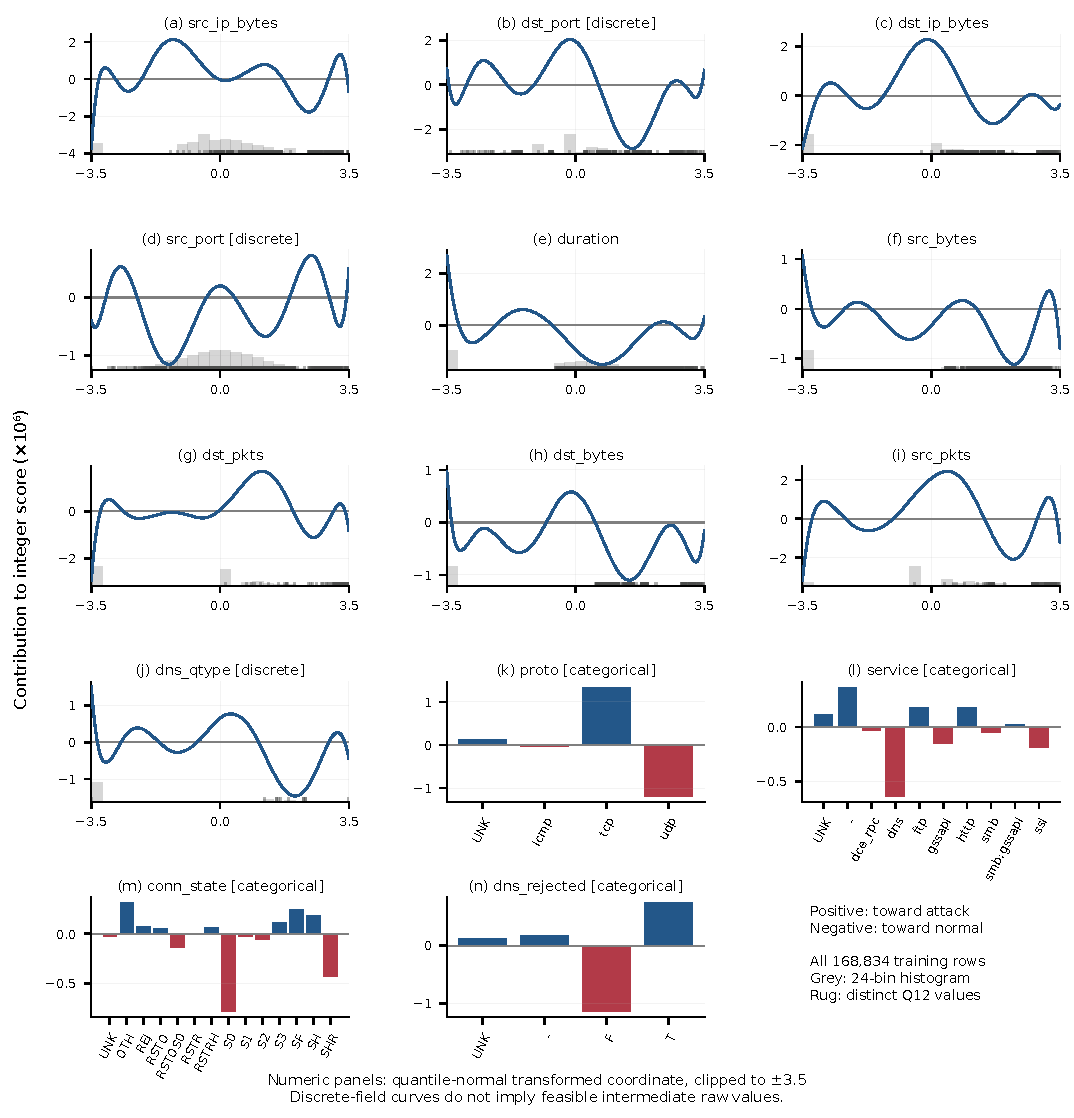
\includegraphics[width=\textwidth,height=0.80\textheight,keepaspectratio]{xai_global.pdf}
\caption{Exact additive terms of the frozen coefficient KAN. Numerical curves use 401 rounded Q12 locations; shaded histograms use 24 bins over all 168,834 training rows, with observed-value rugs. Horizontal numerical coordinates are transformed values clipped to $\pm3.5$. Category labels come from the frozen vocabulary, including UNK. Support is not class-conditioned; vertical values are contributions in millions of integer-score units. Histogram heights are normalized separately in each panel.}
\label{fig:xai-global}
\end{figure*}

Figure~\ref{fig:xai-local} gives three illustrative cases from the historical 200-vector balanced test fixture: the largest predicted-attack score, smallest predicted-normal score, and smallest absolute score. Their indices are 7, 140, and 29, with scores 12,042,992, $-11,561,249$, and 120,232. These rules select illustrations only and are unrelated to model or LUT selection.

\begin{figure*}[!tp]
\centering
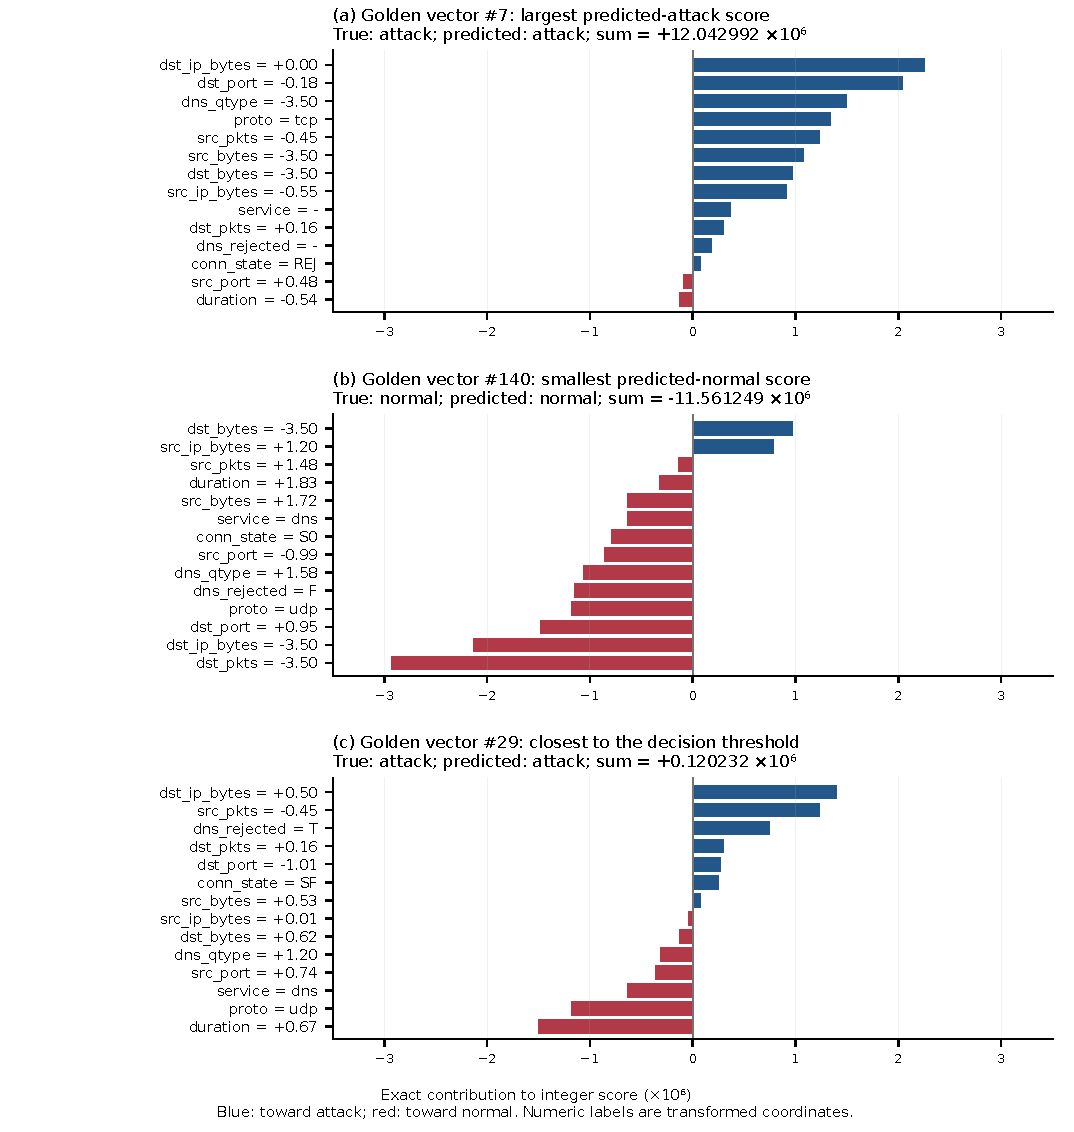
\includegraphics[width=\textwidth,height=0.77\textheight,keepaspectratio]{xai_local.pdf}
\caption{Three predetermined illustrative cases from the historical 200-vector fixture. Bars are all fourteen uncentered contributions in millions of integer-score units; positive values increase the attack score and negative values decrease it. True and predicted classes are shown explicitly. Numerical feature values are transformed coordinates, and case selection is descriptive rather than an explanation-quality test.}
\label{fig:xai-local}
\end{figure*}

This explanation establishes computational fidelity. It does not establish causal attribution or a unique importance ordering: constants can be redistributed among additive functions without changing the total score. Contributions are not centered against a reference population, and unknown-category contributions in the frozen model are nonzero. The same univariate decomposition of original inputs does not apply to the multilayer KAN. The sampled LUT is also additive, but its individual contributions and total score may differ from the coefficient values. The explanations plotted here refer to the coefficient implementation. No physical XAI execution-time or memory claim is made.

\section{Classification Results}
\subsection{Native features and harmonized transfer}
Native TON\_IoT binary cross-validation gives mean F1 values of 0.999136 for LightGBM, 0.998890 for XGBoost, 0.997593 for multilayer KAN, 0.996442 for MLP16, 0.994449 for DT5, and 0.983530 for additive KAN. Full native binary and multiclass results with sample standard deviations are included in Appendix~\ref{app:results}. They show that the compact additive KAN does not dominate predictive quality. Its model-array footprint and exact decomposition are separate properties.

\begin{table*}[t]
\caption{Mean balanced accuracy in the rich harmonized space. The first two columns summarize 50 fits each; the other columns summarize 10 fits each. Joint denotes the equal-domain, normal:attack 1:5 protocol. These conditions differ in training population, sample count, categorical encoding and class weights; they compare fixed pipelines rather than isolate architecture.}
\label{tab:cross}
\centering\small
\begin{tabular}{lrrrrrrr}
\toprule
Model & TON$\to$TON & BoT$\to$BoT & TON$\to$BoT & BoT$\to$TON & Joint$\to$TON & Joint$\to$BoT & Joint$\to$UNSW\\
\midrule
Additive KAN & .9701 & .9934 & .5573 & .6112 & .9432 & .9825 & .3991\\
Multilayer KAN & .9932 & .9971 & .4588 & .6855 & .9811 & .9924 & .3629\\
MLP16 & .9879 & .9426 & .4369 & .7343 & .9296 & .9494 & .3119\\
DT5 & .9828 & .9952 & .5494 & .4597 & .9669 & .9865 & .4081\\
LightGBM & .9963 & .9971 & .4779 & .6964 & .9846 & .9951 & .3884\\
XGBoost & .9947 & .9779 & .5528 & .6487 & .9804 & .9925 & .4193\\
\bottomrule
\end{tabular}
\end{table*}

% Source: work/results/crossdomain_summary_cat.csv; sample SD checked
% against work/results/crossdomain_runs_cat.csv.
\begin{table*}[t]
\centering
\caption{Rich-space single-source balanced accuracy, mean $\pm$ sample SD on the 0--1 scale. In-domain columns summarize 50 fits; transfer columns summarize ten fits (seeds 42--51). The 50:1 attack:normal cap affects training only. Tests retain natural priors; repeat variability does not represent independent networks.}
\label{tab:supp-cross-dispersion}
\footnotesize
\setlength{\tabcolsep}{6pt}
\begin{tabular}{lcccc}
\toprule
Model & TON$\to$TON & BoT$\to$BoT & TON$\to$BoT & BoT$\to$TON \\
\midrule
Additive KAN & $0.9701 \pm 0.0012$ & $0.9934 \pm 0.0010$ & $0.5573 \pm 0.0095$ & $0.6112 \pm 0.0695$ \\
Multilayer KAN & $0.9932 \pm 0.0007$ & $0.9971 \pm 0.0027$ & $0.4588 \pm 0.0548$ & $0.6855 \pm 0.0977$ \\
MLP16 & $0.9879 \pm 0.0016$ & $0.9426 \pm 0.0361$ & $0.4369 \pm 0.0634$ & $0.7343 \pm 0.0144$ \\
DT5 & $0.9828 \pm 0.0015$ & $0.9952 \pm 0.0034$ & $0.5494 \pm 0.0089$ & $0.4597 \pm 0.0107$ \\
LightGBM & $0.9963 \pm 0.0004$ & $0.9971 \pm 0.0031$ & $0.4779 \pm 0.0083$ & $0.6964 \pm 0.0545$ \\
XGBoost & $0.9947 \pm 0.0004$ & $0.9779 \pm 0.0087$ & $0.5528 \pm 0.0269$ & $0.6487 \pm 0.0461$ \\
\bottomrule
\end{tabular}
\end{table*}


Table~\ref{tab:cross} makes the transfer limitation explicit. Although rich in-domain balanced accuracy is generally high, TON-to-BoT means range from 0.4369 to 0.5573. Additive KAN has the largest observed mean in that direction, whereas MLP16 leads BoT-to-TON with 0.7343. This reversal provides no basis for general KAN superiority. Different sampling mechanisms, feature semantics, and class-conditional distributions remain after harmonization.

\subsection{Frozen-model sensitivity to exact row overlap}
\label{sec:duplicate-sensitivity}
A new host-side reanalysis applies the unchanged integer evaluator to the existing canonical test set, separately for the 5,201 exact training matches and the remaining 37,008 rows (Table~\ref{tab:duplicate-sensitivity}). It performs no training, new model selection or hardware run. BA/F1 are 0.9924/0.9965 on the matching rows and 0.9731/0.9808 on the remaining rows, compared with 0.9754/0.9826 overall. Matching rows have higher observed performance, but subgroup difficulty and class composition also differ; this is not a causal estimate of duplicate-induced optimism.

Both LUT sizes retain identical decisions in each subgroup. All three uncertified $L=1025$ decisions and all twelve uncertified $L=513$ decisions occur among rows without an exact match (Table~\ref{tab:duplicate-certificates}). The certificate remains an implementation-agreement result. The remaining rows can still share hosts, sessions, times or model inputs with training; equality after removing labels and identifiers is not tested here. This post-hoc sensitivity analysis neither creates a new independent holdout nor replaces grouped or temporal retraining.

\begin{table*}[t]
\caption{Post-hoc exact-row-overlap sensitivity of the frozen integer model on the canonical TON test set. Coefficients and both fixed LUTs ($L=513,1025$) give identical decisions in every row below. Equality is across all 44 parsed raw columns, including labels and addresses, with the retained missing-value parsing; ``no exact match'' does not mean independent or cleanly deduplicated.}
\label{tab:duplicate-sensitivity}
\centering\footnotesize\setlength{\tabcolsep}{4pt}
\begin{tabular}{lrrrrrrrrrr}
\toprule
Test subgroup & $N$ & Normal & Attack & TN & FP & FN & TP & FPR & TPR & BA / F1\\
\midrule
All & 42,209 & 10,000 & 32,209 & 9,786 & 214 & 896 & 31,313 & .0214 & .9722 & .9754 / .9826\\
Exact training match & 5,201 & 1,634 & 3,567 & 1,609 & 25 & 0 & 3,567 & .0153 & 1.0000 & .9924 / .9965\\
No exact training match & 37,008 & 8,366 & 28,642 & 8,177 & 189 & 896 & 27,746 & .0226 & .9687 & .9731 / .9808\\
\bottomrule
\end{tabular}
\end{table*}

\begin{table}[t]
\caption{Overlap subgroups under the signed LUT-score certificate in~\eqref{eq:signed_threshold_certificate}. $U$ is the number left uncertified; empirical coefficient--LUT decision differences are zero in every row. All uncertified test decisions lie in the no-exact-match subgroup.}
\label{tab:duplicate-certificates}
\centering\footnotesize\setlength{\tabcolsep}{3pt}
\begin{tabular}{lrrrr}
\toprule
Subgroup & $L$ & $N$ & $U$ & Certified\\
\midrule
All & 513 & 42,209 & 12 & 42,197\\
Exact match & 513 & 5,201 & 0 & 5,201\\
No exact match & 513 & 37,008 & 12 & 36,996\\
All & 1025 & 42,209 & 3 & 42,206\\
Exact match & 1025 & 5,201 & 0 & 5,201\\
No exact match & 1025 & 37,008 & 3 & 37,005\\
\bottomrule
\end{tabular}
\end{table}


% Supplemental software study. These are new floating-point models, not the
% frozen checkpoints used for integer certification or hardware measurements.
\subsection{Supplemental endpoint-pair generalization study}
\label{sec:pair-stage2}
To examine sensitivity to the partition and include another additive baseline,
we fitted new models on a fixed endpoint-pair split of the 211,043-row TON\_IoT
source file. Both traffic directions for an unordered pair of source and
destination IP addresses were assigned together; ports were excluded from the
group key. A fixed salted SHA-256 rule assigned pairs to training, validation,
and test buckets in proportions 60:20:20, yielding 119,334, 53,622, and 38,087
rows, respectively. No pair or complete 44-column row crosses these partitions.
This is not a host-, time-, or feature-disjoint split: training and test share
50 hosts, and 2,889 test rows (7.585\%) have transformed model inputs present in
training. The test contains 3,669 normal and 34,418 attack rows and lacks
backdoor, ransomware, and XSS examples.

All models share ten numeric features selected using binary training labels
only, and four categorical fields; preprocessing was fitted only on training. The configurations
were an additive degree-eight KAN, a depth-five decision tree, a 16-unit MLP,
and an additive cubic B-spline logistic GAM with five knots per numeric feature
and no interactions. Unseen categorical values use an all-zero one-hot block;
never-trained KAN category-zero entries were set to zero without changing
training logits. A single-seed validation pilot preceded the fixed five-seed
study; no model, hyperparameter, seed, or threshold was selected from its scores.
The five model seeds were 20260916--20260920; the preprocessing seed was fixed
at 20260916. All twenty fitted checkpoints were frozen before test evaluation,
and the decision threshold remained 0.5. These new floating-point checkpoints
are separate from the frozen integer exports and hardware cohorts.

\begin{table*}[t]
\centering
\caption{Supplemental endpoint-pair test: mean $\pm$ sample standard deviation
over five model seeds on the same 38,087 rows. Standard deviations describe
optimization variation on one fixed split; they are not confidence intervals.
FPR and TPR are percentages.}
\label{tab:pair-stage2}
\small
\begin{tabular}{lccccc}
\toprule
Model & BA & F1 & FPR (\%) & TPR (\%) & AUROC\\
\midrule
Additive KAN & $0.89484\pm0.00022$ & $0.98695\pm0.00009$ & $20.594\pm0.050$ & $99.563\pm0.019$ & $0.98488\pm0.00027$\\
DT5 & $0.68510\pm0$ & $0.96620\pm0$ & $62.687\pm0$ & $99.707\pm0$ & $0.49014\pm0$\\
MLP16 & $0.98885\pm0.00062$ & $0.99798\pm0.00015$ & $2.044\pm0.152$ & $99.815\pm0.039$ & $0.99806\pm0.00044$\\
Spline GAM & $0.97003\pm0$ & $0.99561\pm0$ & $5.724\pm0$ & $99.730\pm0$ & $0.99606\pm0$\\
\bottomrule
\end{tabular}
\end{table*}

The KAN exceeds DT5 in balanced accuracy on this split but remains below both
MLP16 and the spline GAM (Table~\ref{tab:pair-stage2}). Its F1 of 0.98695
coexists with a 20.594\% false-positive rate, which limits deployment usefulness.
For the 35,198 test rows whose transformed inputs are absent from training,
mean KAN BA is 0.89638, F1 is 0.98613, and FPR is 20.248\%; this subgroup has
3,623 normal and 31,575 attack rows. The matching-input subgroup contains only
46 normal rows, so its rates have limited normal-class support. These results
do not establish that additive structure improves detection or that the
canonical-split scores were inflated by leakage: the partition, class mix,
preprocessing fit, and model checkpoints differ. They support a narrower
contribution centered on verifiable integer deployment when an additive score
is required. The five seeds are not independent datasets, and neither the
validation pilot nor these test scores are pooled with the hardware cohort.


\subsection{Joint training and external stress tests}
The corrected validation criterion decreases from $0.97320\pm0.00405$ at ratio five to $0.95230\pm0.00421$ at ratio one hundred. The standard deviation is calculated across ten seed-level averages, after averaging the six models and two validation domains within each seed. Ratio five is the best tested boundary point. Changing the ratio also changes training size, so this grid does not isolate a causal class-balance effect.

Joint models attain mean BA from 0.9296 to 0.9846 on TON and from 0.9494 to 0.9951 on BoT. These values support coverage of both represented source domains under the particular balanced union. They do not establish that pooling alone caused the change: direct-transfer and joint protocols differ in fit sizes, source composition, and train/test partitions.

On UNSW, all joint rich-space means are below 0.42, ranging from 0.3119 to 0.4193. A constant prediction of either class gives BA exactly 0.5. Independent recomputation from the saved confusion counts confirms all six means; 59 of the 60 individual fits are below 0.5, and none predicts a single class throughout UNSW. The saved unseen-category rates are zero. Subsequently recovered source CSVs match the author-reported SHA-256 hashes. An independent implementation reproduced all sixteen supplied harmonized columns for 257,673 rows exactly (4,122,768 value comparisons), and every raw binary label agrees with its attack category. This rules out a label or numerical-transformation discrepancy on the checked raw-to-cache segment, but does not recover the historical fitted preprocessors, models or aligned scores.

The saved rich-space AUROC values also diagnose a ranking failure: 57 of 60 runs are below 0.5. Means range from 0.2777 for MLP16 to 0.4140 for XGBoost (Table~\ref{tab:unsw-auroc}); thus the negative result is not confined to the fixed threshold. These are reaggregated historical metrics, not ROC curves recomputed from predictions. Without row-level scores we cannot independently recalculate AUROC or attribute the errors, and no output or label reversal is used to repair target results.

\begin{table}[t]
\caption{Historical rich-space UNSW AUROC, mean and sample SD across ten saved seed records per model. Aggregation was rechecked; absent row-level scores prevent independent recomputation of each AUROC.}
\label{tab:unsw-auroc}
\centering\footnotesize
\begin{tabular}{lcc}
\toprule
Model & AUROC & Runs below 0.5\\
\midrule
Additive KAN & $0.3242\pm0.0567$ & 10/10\\
Multilayer KAN & $0.3301\pm0.0555$ & 10/10\\
MLP16 & $0.2777\pm0.0388$ & 10/10\\
DT5 & $0.3714\pm0.0698$ & 10/10\\
LightGBM & $0.3702\pm0.0723$ & 9/10\\
XGBoost & $0.4140\pm0.0749$ & 8/10\\
\bottomrule
\end{tabular}
\end{table}


Reconstructing the balanced joint-source cohorts under the retained sampling code gives a more specific diagnostic than comparing full source populations. Across all ten reconstructed cohorts, protocol \texttt{other} occurs in 35--42 observations, all normal; in UNSW the same mapped category contains 37,919 attacks among 41,916 observations (90.46\%). Table~\ref{tab:unsw-category-shift} also shows changes in the class associations of TCP, UDP and \texttt{closed}. By contrast, \texttt{established} is relatively associated with normal traffic in both the reconstructed mixture and UNSW. These are descriptive properties of the data. Missing historical model outputs prevent assigning a causal contribution to each change; Appendix~\ref{app:data-checks} records reconstruction assumptions, feature selection and further checks.

Reduced-space joint models on the CIC subset yield $0.492754\pm0.040544$ for LightGBM, $0.509947\pm0.008238$ for XGBoost, $0.500243\pm0.053045$ for multilayer KAN, $0.414416\pm0.071708$ for DT5, $0.472501\pm0.040057$ for MLP16, and $0.497395\pm0.010734$ for additive KAN. The proxy adapter combines distribution shift with measurement and mapping mismatch: all non-TCP observations receive the \texttt{incomplete} state after the TCP-flag rules. Neither external target establishes a robustness benefit or isolates an intrinsic KAN limitation.

The sanity check also found a resume-related aggregation defect: the archived rich-space UNSW DT5 pooled confusion matrix contained nine seeds, while the per-fit table contained all ten. Reconstructing the pooled matrix from all ten records corrects this artifact; the reported mean BA remains 0.4081494. Recovered JSONL checkpoints independently corroborate all 420 current model--seed--domain evaluation records (180 rich and 240 reduced) and the 42 complete pooled matrices. The corrected aggregation uses the complete merged run table, with regression checks for identical seed sets and pooled counts. These records strengthen the provenance of the aggregates; they do not supply row-aligned scores or explain the below-0.5 mean.

The reported dispersions describe repeated training, subsampling, and random splitting of the available observations. Seeds do not constitute independent networks; fold estimates also share observations. We therefore use descriptive mean and sample SD, without significance claims based on treating these repeats as independent deployment environments.

\section{Physical Microcontroller Evaluation}
\subsection{Devices, implementations, and timing boundary}
The controlled factorial experiment in Section~\ref{sec:c3followup} is the primary comparison for the ESP32-C3 coefficient--LUT and memory-placement question. Section~\ref{sec:hw500} reports sustained-batch time and USB energy for the same 500-flow hardware cohort, and Section~\ref{sec:ram500} reports separately instrumented RAM components. The original five-implementation comparison and intermediate diagnostic are retained as supporting experiments with distinct boundaries.

The devices are an Arduino Mega 2560 R3 with a 16-MHz ATmega2560 and an ESP32-C3 board with a SuperMini layout. The ESP probe identified revision 0.4, 4 MB of embedded Flash, and the firmware reported a 160-MHz CPU clock. Both boards were USB powered; Fig.~\ref{fig:energy-setup} shows the two instrumented measurement setups side by side. Builds used PlatformIO Core 6.1.19. The Mega toolchain records atmelavr 5.1.0, Arduino AVR 5.2.0, and GCC 7.3.0. ESP builds use espressif32 6.12.0, Arduino 2.0.17, and GCC 8.4.0; the effective final optimization option is \texttt{-Os}. Recorded commands and binaries define the measured configurations.



The five implementations are the additive coefficient KAN, its selected sampled LUT, the multilayer coefficient KAN, an integer MLP16, and DT5. Each uses its frozen model-specific input adapter. The MLP implementation substitutes category-table lookups for explicit one-hot construction; the tree uses a compact node table. These baseline kernels are measured on the same boards and observations. Boosting results remain part of the dataset-scale comparison and are not assigned new hardware measurements in this study.

For the short-kernel experiments, the common cohort contains 500 distinct original TON flows, comprising 250 normal and 250 attack observations in interleaved order. Source identifiers and order are identical across all five implementations and both devices. Preprocessing is performed offline with each model's frozen adapter. Common raw observations do not imply an identical transformed input matrix for models with different adapters.

Table~\ref{tab:protocol-map} separates six hardware protocols. The matched factorial experiment is the primary ESP32-C3 coefficient--LUT comparison. In the original five-implementation experiment the LUT was 7.58\% slower on ESP32-C3 under a different protocol; the cause remains unresolved. Appendix~\ref{app:historical-hardware} retains that unfavorable result, the five-model timing table and figure, and the intermediate locality diagnostic. On Mega, the original experiment measured a $5.746\times$ coefficient-to-LUT speedup. The common 500-flow cohort produced 18 errors for both additive representations, 6 each for multilayer KAN and MLP16, and 9 for DT5; agreement with an implementation reference is distinct from detection quality.

\begin{table*}[t]
\caption{Four distinct ESP32-C3 protocols. All use one physical board at 160 MHz and prepared native TON\_IoT inputs; no row is pooled with another. Placement denotes the inference kernel and model parameters. Retained records establish build settings and observed execution, not hardware-wide guarantees.}
\label{tab:protocol-map}
\centering\scriptsize\setlength{\tabcolsep}{3pt}
\begin{tabular}{p{2.0cm}p{3.2cm}p{2.5cm}p{3.5cm}p{5.3cm}}
\toprule
Experiment & Timer and measured endpoint & Code / parameters & Inputs and repeat structure & Warmup, harness and interpretation\\
\midrule
Original five models (Appendix~\ref{app:historical-hardware}) & \texttt{micros()}, 1-$\mu$s grid; one call through binary decision & Original application placement; parameters in Flash & 500 flows; five reset-separated passes per model & 64 warmup calls per pass; prepared input copy and serial/reference checks excluded. LUT mean is 7.58\% higher than coefficients.\\
Intermediate diagnostic (Appendix~\ref{app:historical-hardware}) & Cycle counter; integer logit, or amortized 32-call block with loop and stores & IRAM / Flash or DRAM & 500 flows; five ordered passes in one boot & 2,000 warmup calls per block, balanced four-condition order; interrupts enabled. \texttt{same32} repeats one input within each block.\\
Matched factorial (primary; Section~\ref{sec:c3followup}) & Cycle counter; one call and binary threshold & Flash or IRAM / Flash or DRAM & 500 flows; eight reset-separated passes; eight conditions & Full 500-flow warmup per condition; Williams order; interrupts enabled, serial outside blocks, \texttt{-Os}, LTO disabled. Flash-code/DRAM-parameter LUT speedup: $1.706\times$.\\
USB-energy pilot (Section~\ref{sec:energy-pilots}) & Complete MCU batch duration / call count; central-window USB power & Original pilot Flash parameters; separate linked applications & First 20 flows repeatedly cycled; two acquisitions per model, one boot per C3 pair & Warmup and count calibration before roughly 120 s of active loop; inference, indexing, checksums and interrupts included. Wi-Fi/Bluetooth not initialized; no explicit yield. Coefficient/LUT time ratio: $1.567\times$.\\
\bottomrule
\end{tabular}
\end{table*}

The matched-factorial upload command specifies DIO, 80 MHz and 4 MB Flash. These are recorded upload settings, not an independent runtime Flash-clock measurement. The archived build pins espressif32 6.12.0, Arduino package 3.20017.241212, a 160-MHz CPU, \texttt{-Os}, \texttt{-fno-lto}, \texttt{-fno-jump-tables} and \texttt{-fno-tree-}\allowbreak\texttt{switch-conversion}. A corresponding \texttt{sdkconfig} was not retained, so cache-line and RTOS-tick settings are not inferred. Delays in the harness occur outside timed blocks.


\subsection{Reset-separated code and parameter placement experiment}
\label{sec:c3followup}
\begin{table*}[t]
\centering\footnotesize\setlength{\tabcolsep}{4pt}
\caption{ESP32-C3 follow-up with a common binary-decision timing boundary. Each condition comprises 500 fixed source flows in each of eight reset-separated passes. Mean times and sample standard deviations of the eight pass means are in $\mu$s. The 95th percentile uses the nearest rank among 4000 calls. Ratios compare coefficient and LUT implementations at the same code and parameter placement. An asterisk denotes a pass-mean SD below $0.0001~\mu$s. All means and p95 values are in $\mu$s.}
\label{tab:c3_followup}
\begin{tabular}{llrrrrr}
\toprule
Code & Parameters & Coeff. & LUT & Speedup & Coeff. p95 & LUT p95\\
\midrule
Flash & Flash & $5.1690\pm0.0062$ & $3.6064\pm0.0114$ & $1.433\times$ & 5.1375 & 5.9375\\
Flash & DRAM & $5.1364^{*}$ & $3.0104\pm0.0043$ & $1.706\times$ & 5.1125 & 3.0000\\
IRAM & Flash & $5.1364^{*}$ & $3.3295\pm0.0096$ & $1.543\times$ & 5.1125 & 4.6438\\
IRAM & DRAM & $5.1447\pm0.0043$ & $3.0339^{*}$ & $1.696\times$ & 5.1438 & 3.0313\\
\bottomrule
\end{tabular}
\end{table*}

The follow-up used a fixed $2\times2\times2$ design: coefficient or sampled-LUT representation, code in Flash or IRAM, and parameters in Flash or DRAM. Eight reset-separated passes followed a Williams order that placed every condition once in every block position and covered every ordered pair of neighbouring conditions once. Each condition received a complete 500-flow warmup followed by 500 timed decisions on the same prepared inputs. Serial transmission, parameter initialization, warmup, and validation were outside the single-call intervals. The common cycle-counter boundary included a kernel call and the binary threshold; interrupts remained enabled. All 4096 empty-timer samples were one cycle, without overhead subtraction. Independent cycle-counter checks were consistent with the configured 160~MHz clock.

Independent ELF inspection confirms that the Flash and IRAM copies are byte-identical within each family: 346 bytes for the coefficient kernel and 206 bytes for the LUT kernel. Thus the code-placement comparison does not change the arithmetic instruction sequence. The timer has two cycle-counter reads surrounding the indirect kernel call and the binary threshold; the prediction store follows the second read. The released source and frozen parameter arrays agree with the uploaded build artifacts. Compilation uses the same pinned GCC 8.4.0 toolchain with \texttt{-Os} and LTO disabled.

The LUT was faster at all four matched placements (Table~\ref{tab:c3_followup}). The lowest observed mean was $3.0104~\mu$s with code in Flash and parameters in DRAM, compared with $5.1364~\mu$s for coefficients at the same placement: a $1.706\times$ speedup and a 41.392\% reduction. Moving LUT parameters from Flash to DRAM reduced its mean time by 16.527\% with Flash code and by 8.877\% with IRAM code. Moving LUT code to IRAM helped when parameters remained in Flash (7.679\% reduction), but increased the mean by 0.783\% when parameters were already in DRAM. Flash/Flash LUT improved the mean but had a higher p95 than coefficients; placing LUT parameters in DRAM reduced p95 to $3.0000~\mu$s. The maximum recorded call in this fastest condition was $9.0375~\mu$s, so the percentile is not a worst-case execution-time guarantee.

A paired factorial analysis uses one mean for each condition and reset-separated pass. Averaged across the four placements, the LUT-minus-coefficient contrast is $-1.9016~\mu$s, with SD $0.0040~\mu$s across the eight pass contrasts. Moving LUT code from Flash to IRAM reduces mean latency by $0.2769~\mu$s with Flash parameters but increases it by $0.0236~\mu$s with DRAM parameters; both directions occur in all eight passes. Appendix~\ref{app:factorial} gives the seven factorial contrasts. These repeated-block effects describe this board and protocol; they do not identify the cause of the earlier protocol discrepancy.

All 32\,000 timed binary decisions matched the frozen compiled-C references. Separately, all 32\,000 logits recorded during untimed post-block replay matched the representation-specific references. Each 500-flow condition retained 18 classification errors; execution agreement is distinct from detection accuracy. The device also reported zero mismatches in preflight and pre/post-block checks. The eight passes concern one board and a fixed, warmed input sequence; small pass-mean deviations do not describe variation across devices. Rare excursions of approximately 965 cycles were retained without causal attribution. The benchmark measures prepared-feature inference, not preprocessing, energy, cold-start performance, or peak runtime SRAM. The DRAM LUT payload alone is 20\,554 bytes versus 254 bytes for coefficients. These results establish an effective deployment choice under the common follow-up protocol; they do not establish a unique cause of the earlier protocol discrepancy or update the historical MLP/DT5 timing comparison.


\begin{figure*}[t]
\centering
\begin{minipage}[b]{0.47\textwidth}
\centering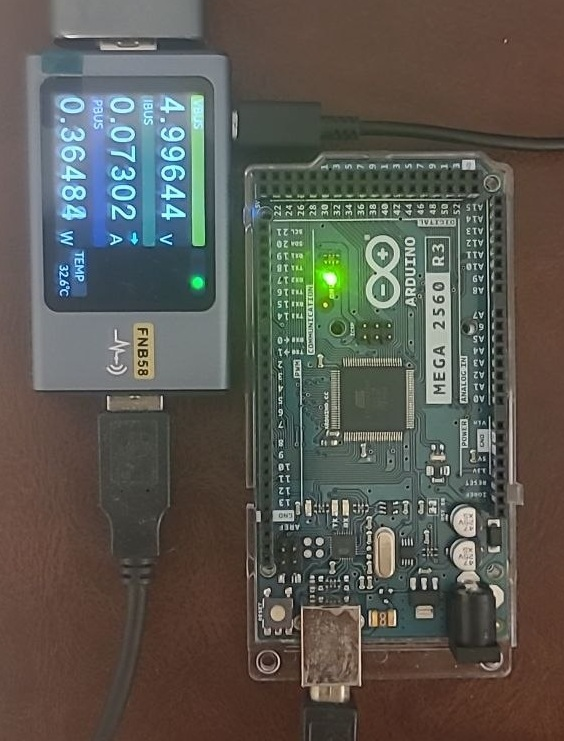
\includegraphics[height=5cm]{Mega_measurement.jpg}\\[-1pt]
{\small (a) Arduino Mega 2560}
\end{minipage}\hfill
\begin{minipage}[b]{0.47\textwidth}
\centering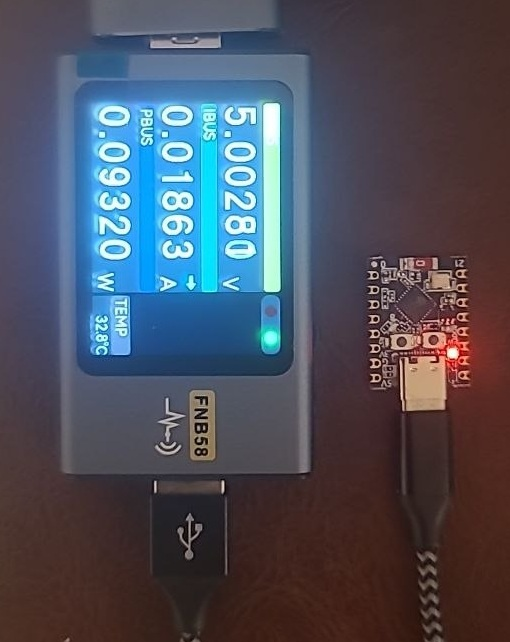
\includegraphics[height=5cm]{C3_measurement.jpg}\\[-1pt]
{\small (b) ESP32-C3}
\end{minipage}
\caption{USB measurement setups for (a) Mega 2560 and (b) ESP32-C3. Displayed voltage, current and power are instantaneous connection snapshots; quantitative results use archived active-window records. The photographs illustrate the connections, without identifying a particular acquisition.}
\label{fig:energy-setup}
\end{figure*}

\subsection{Time and USB energy on the common 500-flow workload}
\label{sec:hw500}
We next used one common 500-flow cohort (250 normal and 250 attack flows) for both timing and energy on the same Mega 2560 and ESP32-C3 boards. These are the historical frozen models; the newly fitted pair-disjoint models were not exported for this campaign. Each board completed a separate coefficient pilot and five blocks containing the five models in a prespecified cyclic order, giving five technical repetitions per configuration. The pilot was excluded from the reported means. Each run used a fresh upload/reset, 500 warm-up predictions, calibration of the batch count to approximately 120\,s, and at least 30\,s of stabilization. Every prepared row was read from Flash into a small RAM buffer, evaluated, and added to a prediction checksum. The timed batch excludes feature extraction, packet capture, serial output, LED markers, warm-up and calibration. Its duration divided by the number of completed predictions is a batch-average processing time, not a distribution of individual-request latencies.

One continuous FNB58 record per board covered the pilot and 25 subsequent runs. Positive LED marker groups before and after each run were associated with the host chronology; an affine fit of twelve MCU-timestamped edges registered each active interval to the stored power trace. We integrated VBUS$\times$IBUS by the trapezoidal rule over the full mapped active interval and divided by its completed prediction count $N$:
\begin{equation}
\widehat E_{\rm iter}=\frac{1}{N}\int_{t_0}^{t_1}V(t)I(t)\,dt,
\qquad \overline t_{\rm iter}=\frac{T_{\rm MCU}}{N}.
\label{eq:hw500-energy}
\end{equation}
Boundary samples are linearly interpolated. Sustained repeated inference is also used by MLPerf Tiny, while ULPMark-CM measures active CPU energy~\cite{Banbury2021MLPerfTiny,EEMBCULPMarkCM}; our whole-board USB protocol is not a reproduction of either benchmark. Thus the time and energy in Table~\ref{tab:hw500-energy} refer to the same batch and include the complete downstream USB-powered board and connection. Adjacent idle powers are retained as diagnostics but are not subtracted. In particular, four Mega configurations had negative signed idle-subtracted differences; these are not interpreted as negative inference energy. The unexplained NRG channel discrepancy (approximately one quarter of the VBUS$\times$IBUS integral) remains documented, and NRG is not used or rescaled.

\begin{table*}[t]
\centering\small
\caption{Common 500-flow hardware workload: mean time and whole-board USB energy per iteration, both obtained from the same complete active batch. Five technical repetitions per model and board; energy is mean $\pm$ sample SD. This dispersion describes technical repeatability, not absolute accuracy. The separate coefficient pilot is excluded.}
\label{tab:hw500-energy}
\begin{tabular}{lrrrr}
\toprule
Model & \multicolumn{2}{c}{Mega 2560} & \multicolumn{2}{c}{ESP32-C3} \\
 & Time ($\mu$s) & Energy ($\mu$J) & Time ($\mu$s) & Energy ($\mu$J) \\
\midrule
Coefficient KAN & 1412.4 & $498.4\pm0.8$ & 5.892 & $0.9874\pm0.0004$ \\
LUT KAN & 258.83 & $92.16\pm0.13$ & 4.961 & $0.8590\pm0.0007$ \\
MLP16 & 1344.4 & $477.3\pm0.7$ & 20.592 & $3.5263\pm0.0040$ \\
Multilayer KAN & 12321.8 & $4367\pm4$ & 55.752 & $9.6408\pm0.0102$ \\
DT5 & 33.035 & $11.884\pm0.010$ & 1.536 & $0.2643\pm0.0002$ \\
\bottomrule
\end{tabular}
\end{table*}

LUT reduced the batch-average time relative to coefficient KAN by factors of 5.457 on Mega and 1.188 on C3; the corresponding whole-board energy ratios were 5.407 and 1.149. DT5 remained the fastest and lowest-energy implementation in this workload. All five recorded Mega durations were identical within each configuration; this is zero observed variation in stored batch durations, not zero timing uncertainty. The new series removes the workload mismatch between the earlier twenty-flow energy pilots and the 500-flow timing cohort. Those historical protocols remain separate and are not pooled with these results. The new C3 result does not isolate the cause of the earlier protocol's 7.58\% LUT slowdown.

Neither the meter nor the clocks were independently calibrated. The 0.1\,s storage grid does not establish 10\,Hz measurement bandwidth: the observed marker response was about 1\,s. The maximum marker-fit residual was 0.102\,s on Mega and 0.142\,s on C3. A common shift of both integration endpoints over $\pm2$\,s changed the estimates by at most 0.034\% and 0.605\%, respectively. These are registration diagnostics, not a complete uncertainty budget. Means and sample SD describe technical repeatability on one board of each type and do not establish absolute accuracy, variation between devices, isolated processor energy, or end-to-end IDS cost.


\subsection{Model arrays, firmware, and SRAM}
\begin{table*}[t]
\caption{Original five-implementation protocol: memory accounting in bytes. Model arrays exclude code and fixtures. Mega Flash is the linked program-use figure; ESP Flash is the actual application BIN length. These platform-specific image measures include the benchmark and framework. Linked SRAM is not peak runtime usage.}
\label{tab:memory}
\centering\small
\begin{tabular}{lrrrrrr}
\toprule
& & \multicolumn{2}{c}{Mega 2560} & \multicolumn{3}{c}{ESP32-C3}\\
\cmidrule(lr){3-4}\cmidrule(lr){5-7}
Implementation & Model arrays & Flash & Static data & App BIN & DRAM data & Shared SRAM extent\\
\midrule
KAN coefficients & 254 & 20,480 & 217 & 280,352 & 13,940 & 62,080\\
KAN sampled LUT & 20,554 & 40,286 & 217 & 295,088 & 13,940 & 62,080\\
Multilayer KAN & 5,244 & 26,434 & 217 & 280,672 & 13,940 & 62,080\\
MLP16 & 760 & 20,442 & 217 & 280,224 & 13,940 & 62,080\\
DT5 & 285 & 21,452 & 217 & 280,032 & 13,932 & 62,064\\
\bottomrule
\end{tabular}
\smallnote{ESP also reserves 48,128 bytes for IRAM code and alignment within the shared SRAM extent; the aliased \texttt{.dram0.dummy} range is counted once. A separate 32-byte RTC allocation is excluded from the shared SRAM extent. These original applications have no runtime stack/heap measurements; the later instrumented applications are reported separately in Table~\ref{tab:ram500}.}
\end{table*}

Table~\ref{tab:memory} reports the original five-implementation applications and separates quantities that should not be conflated. The 254-byte coefficient model is the smallest declared model-array representation among the five frozen implementations. However, the complete Mega coefficient benchmark uses 20,480 bytes of Flash, and the corresponding ESP application BIN is 280,352 bytes. The sampled-LUT increase in model arrays is only one contributor to the change in total image size.

Mega linked static data occupy 217 bytes for every application. Stack allocations and heap activity are not captured by that figure. On ESP32-C3, the data-only summary reports 13,940 bytes for four models and 13,932 for DT5, but the linker also reserves 48,128 bytes for instruction RAM, including alignment. The shared SRAM extent through the heap-start boundary is 62,080 or 62,064 bytes, with aliasing counted once. Thus a data-only figure cannot support an 18-KB total runtime SRAM claim. Likewise, the Mega build summary cannot establish a 2-KB runtime peak. Section~\ref{sec:ram500} adds observed runtime components for separate diagnostic applications, without asserting an exact whole-system SRAM peak.

The eight-condition follow-up application contains both DRAM parameter copies (20,808 bytes), descriptors, and measurement buffers. Its application BIN is 307,792 bytes; linked DRAM data and BSS occupy 57,348 bytes, and the shared SRAM address extent through the heap boundary is 105,992 bytes including IRAM and alignment. These figures describe the combined measurement application. The recorded initialization interval of 1466--1499 microseconds includes model, input, and reference copies plus descriptor setup, so it does not isolate LUT-copy cost.

Table~\ref{tab:pilot-memory} separately records the energy-pilot applications on both boards. Their larger data allocations include the twenty prepared inputs and the acquisition harness; they do not replace the original application sizes in Table~\ref{tab:memory}. The MLP model representation is 760 bytes, while its separately linked parameter objects total 756 bytes because the compiler embeds the four-byte output bias in instructions. The instruction-embedded value was checked against the frozen source. All five ESP32-C3 pilot applications additionally reserve 47,906 bytes of IRAM code and 222 bytes of alignment outside the data/BSS totals. No pilot result establishes a stack or heap peak.

\subsection{Observed RAM components in a separate instrumented workload}
\label{sec:ram500}
The RAM500 campaign uses the frozen models and the same 500 prepared hardware inputs in separate diagnostic applications. Each model is evaluated after three fresh uploads, with three full passes per upload. All 22,500 reference comparisons per board agree, and all post-baseline positive controls pass. These are repeated executions of 500 observations, not additional detection-quality samples. The baseline includes prepared-row loading, prediction, reference checking and observed interrupt activity; diagnostic reporting and positive controls follow the saved baseline.

On Mega, static SRAM is 335 bytes for every model, including the reusable input buffer. Wrapped allocator counts are zero throughout each baseline, and the heap boundary is unchanged. The observed stack depths in Table~\ref{tab:ram500} are identical across all three uploads. A positive control allocates and frees 128 requested bytes, changing the heap boundary by 130 bytes and then restoring it. A separate stack control also passes. These checks establish that the probes respond to known allocations; they do not prove the maximum stack depth over every possible input or interrupt schedule.

\begin{table}[t]
\caption{RAM500 observed stack components (bytes), over three fresh uploads per model. Mega static SRAM is 335 bytes and C3 static DRAM data/BSS is 15,312 bytes for every row. C3 ranges are lifetime task watermarks whose maxima were already reached before inference in every run. The columns have different scopes and must not be summed into a global Peak RAM estimate.}
\label{tab:ram500}
\centering\footnotesize
\begin{tabular}{lrr}
\toprule
Implementation & Mega stack depth & C3 loop-task use\\
\midrule
KAN coefficients & 93 & 1584\\
KAN sampled LUT & 80 & 1504--1584\\
Multilayer KAN & 208 & 1504\\
MLP16 & 95 & 1584\\
DT5 & 46 & 1504--1584\\
\bottomrule
\end{tabular}
\end{table}

C3 task watermarks and heap observations follow the ESP-IDF 4.4.7 API semantics~\cite{EspressifFreeRTOS447,EspressifHeap447}: task lifetime stack use and sampled heap state have different scopes. On C3, linked static DRAM data/BSS occupies 15,312 bytes and IRAM code plus alignment occupies 48,128 bytes. The loop task reserves 8,192 bytes. Its pre-workload and post-workload lifetime stack watermarks are identical in every run. Thus the observed 1,504--1,584-byte task use cannot establish a model-specific inference-stack advantage. Internal 8-bit heap snapshots report 309,800 free and 20,588 allocated bytes both before and after each workload. Unchanged snapshots do not exclude intervening transient allocations. A 512-byte control allocation reduces free heap by 528 bytes and is fully released. A separate control task changes its free stack watermark from 3,920 to 3,244 bytes. All fifteen C3 runs pass both controls.

The task-stack reservation is already part of allocated heap and must not be added again. These observations concern diagnostic firmware, not the energy applications or a complete IDS. Finite-workload watermarks, static sections and heap snapshots do not establish an exact whole-system or universal worst-case peak. Repeating the same protocol would refine repeatability without removing that scope limitation. The retained audit gives per-upload values, actual binaries, source identities and raw control traces.


\subsection{Artifact checks}
The archived records include application sources, build commands, toolchain packages, binaries, upload logs, raw serial observations, and source-flow identifiers. ESP application images were checked against their ELF sections and upload addresses. A separate readback after the original five-implementation measurement series matched the complete compiled bootloader prefix, partition-table bytes, OTA reference bytes, and the final DT5 application. Unexplained non-erased bytes after the compiled bootloader remain outside that equality claim. This readback records the observed post-series state, not continuous attestation of every earlier application execution.

\section{Discussion and Limitations}
The 254-byte additive coefficient representation exposes its exact computational terms and supports a measurable time--storage trade-off. Its sampled LUT reduces kernel latency by a factor of 5.746 on Mega 2560. The ESP32-C3 placement experiment establishes a 1.706-fold coefficient-to-LUT speedup with code in Flash and both parameter sets in DRAM, using the same binary-decision timing boundary. Moving the LUT code to IRAM does not improve this DRAM result. The matched-cohort HW500 study measures batch time and energy together; coefficient-to-LUT whole-board energy falls by about 81.5\% on Mega and 13.0\% on ESP32-C3. These values include prepared-row loading and loop work. They neither inherit the short-kernel boundary nor reproduce the smaller twenty-input pilot, whose results remain in Appendix~\ref{app:energy-details}. The original ESP32-C3 protocol showed no LUT gain, while the intermediate diagnostic showed sensitivity to repeated-input locality. The representation choice therefore involves the processor, memory placement, and execution protocol. DT5 remains faster in the original five-implementation experiment, while boosting achieves the strongest native-feature predictive results. The coefficient KAN saves only 31 parameter bytes relative to DT5 (254 versus 285 bytes), and DT5 makes fewer errors on the common 500-flow cohort (9 versus 18). These observations give no accuracy--latency justification for replacing DT5 with the additive KAN in the measured setting. The additive model instead provides the fixed score structure on which we study export verification and the coefficient--LUT trade-off. The new endpoint-pair-disjoint comparison reinforces this scope: additive KAN exceeds DT5 in that separate fit but falls below both GAM and MLP16, with a 20.59\% normal-traffic false-positive rate. Its attack F1 of 0.987 therefore does not establish operational suitability.

The external stress tests give poor performance for the evaluated pipelines; their interpretation also depends on adapter validity. Harmonized quantities reduce explicit field mismatch, but they do not make data collection, observation units, attack behavior, or normal traffic equivalent. Joint-source training gives higher scores on the represented sources than on UNSW or the reduced CIC target. The verified UNSW raw-to-cache transformation narrows the diagnosis, while the reconstructed balanced cohorts expose source--target association changes. Their effects on historical model errors remain unresolved without fitted objects and row-aligned scores. Those results motivate caution about deploying a frozen source classifier in a new network; they are not repaired by interpreting high source-domain F1 as robustness.

A concrete use case is model maintenance when a separate contribution from every transformed input must be recorded and an exported implementation must be checked against a frozen score reference. The additive representation supplies these arithmetic terms directly, and its univariate edge errors can be exhaustively enumerated before deployment. Choosing it for this requirement would still require acceptable detection quality on the intended network and validation that the records help the intended users. Neither condition is established for a new deployment here. The contributions are uncentered terms, not causal effects or a unique ranking of feature importance. We assess computational inspectability and export agreement; human understanding, regulatory acceptance and operational benefit have not been measured. Additive explainability itself is established prior work.

Several limits constrain inference. Historical test inspection precludes describing these targets as untouched confirmation. Historical random observation-level splits retain content overlap in the checked canonical TON split. The new endpoint-pair split removes repeated endpoint pairs but shares hosts and some transformed inputs across train and test; it is not host- or time-disjoint and omits three attack types from its test subset. BoT has only 477 normal observations, with 95 in each joint outer test, so normal recall is based on a small minority pool. Repeated seeds reuse observations. Baselines differ in categorical encoding and weighting. The inherited compact configurations are not demonstrated optima. The two feature families used for hardware and transfer are different, and the hardware cohort is balanced and much smaller than the full test population.

The device experiments establish prepared-feature execution on one unit of each board type. The HW500 study adds descriptive whole-board energy estimates and time for a common sustained 500-flow workload; five technical runs per model do not establish variation across independent devices or networks. The separate RAM500 study reports static allocations, observed stack watermarks and heap observations. On C3, the loop-task lifetime stack maximum predates inference in every accepted run, so it cannot rank model-specific stack demand. No exact whole-system RAM peak, live traffic processing, long-term thermal behavior or performance under radio and application contention is measured. Instrument accuracy and MCU clock error were not independently calibrated; recording-grid resolution and observed repeatability do not constitute an uncertainty budget. Exact additive explanations describe arithmetic, not causal security mechanisms. These limits delimit the contribution without substituting host or simulator estimates for physical measurements.

\section{Conclusion}
For the frozen additive KAN, finite-domain enumeration connects a sampled LUT to the exact integer coefficient evaluator, including its rounding rules. Signed edge-error extrema sharpen the symmetric bound and certify 42,206 of 42,209 test decisions for the 20,554-byte table. All test decisions agree empirically. The 10,314-byte alternative leaves twelve decisions uncertified; the extra storage reduces uncertainty without establishing unconditional lossless compilation. These retrospective checks leave the training-only selection and measured kernels unchanged.

The original Mega experiment measured a $5.746\times$ coefficient-to-LUT speedup. The controlled ESP32-C3 experiment measured $5.136$ versus $3.010~\mu$s with Flash code and DRAM parameters, a $1.706\times$ speedup. Its factorial contrasts show a code--parameter placement interaction; they do not identify the cause of the earlier protocol discrepancy. All 32,000 timed decisions in that experiment matched the compiled references. The HW500 series pairs whole-board energy with batch time on the common 500-flow cohort: coefficient and LUT estimates are about 498 and 92.2~$\mu$J per iteration on Mega, and 0.987 and 0.859~$\mu$J on ESP32-C3. Separate RAM500 runs pass all reference and positive-control checks and report observed memory components, without an exact whole-system peak. These studies complement the short-kernel observations while preserving distinct measurement boundaries. Additive score decomposition remains exact but is neither uniquely interpretable nor empirically shown to improve analyst decisions. Cross-dataset stress tests show poor performance. Exact raw-to-cache checks and reconstructed source cohorts document category--label association changes on UNSW, while their model-level effects remain unresolved. The result is a reproducible agreement analysis and a measured implementation trade-off, with workload-specific energy and memory observations. It establishes neither superior detection nor universal energy efficiency or worst-case memory use.

\section*{Reproducibility and Data Availability}
The author's baseline code is available at \url{https://github.com/emanuelepiodebernardis/kan-ids-v2}, with the checked baseline identified by commit \href{https://github.com/emanuelepiodebernardis/kan-ids-v2/commit/df72c7764874efb8de13383d265e3ff0a8ba937c}{\texttt{df72c7764874}}. The accompanying release candidate preserves corrected selection protocols, frozen model headers, transformed inputs, common cohort identifiers, run-level metrics, raw hardware archives and independent verification scripts. Retained analyses include signed-error and factorial checks, hash-matched UNSW and TON source-to-cache verification, reconstructed joint-cohort associations and a canonical-split duplicate check. Newly recovered native pre-Q12 inputs, JSONL checkpoints and AVR probe objects support the paired export and provenance checks reported here. Their identities and independently checked quantities are recorded in verification receipts. The hardware checkpoint additionally preserves all twenty original power records and run archives, exact delivered sources, actual ELF/HEX/BIN files, and per-record marker alignment and integration results. Separate audits verify provenance, executed loops and energy arithmetic. A manuscript-specific evidence extract links its tables to those accepted records. The new pair-disjoint study additionally preserves fitted preprocessors, floating models, split identities and row-level predictions. These artifacts belong to the new study; the historical joint fitted models, preprocessors and row-aligned scores remain unavailable.

The release artifact maps for v0.15 and the historical v0.12 revision link each central claim to its input hashes, analysis command and expected outputs. They distinguish arithmetic replay on prepared inputs, reaggregation of historical metrics, conditional preprocessing recovery and physical-measurement provenance. The exact-row subgroup analysis evaluates frozen inputs without fitting. The separate endpoint-pair study comprises twenty new floating fits; its metrics are independently recomputed from 761,740 saved test predictions. HW500 retains two continuous meter records and per-run timing/provenance, and RAM500 retains fifteen accepted uploads per board with reference comparisons and instrumentation controls. The release identifies the source versions of each accepted series and retains failed instrumentation attempts as excluded diagnostic records. A complete fitted raw-flow-to-decision pipeline is not established for arbitrary new traffic. The source CSVs, supplied caches, analysis inputs and scripts are identified by hashes in the accompanying verification package. The recovered UNSW CSVs came from a public mirror and match the hashes reported for the historical files; hash equality does not independently establish which bytes the original fitted processes consumed. Manuscript archives contain the LaTeX sources, bibliography, figures and build scripts. Public archival deposition of the revised software and physical records remains pending; the public baseline must not be mistaken for that revised release. Dataset use remains subject to the original providers' terms.

\appendices
\section{Exact Cubic Integer Basis}
\label{app:arithmetic}
For numerical input $q_i$, define $u_i=16\operatorname{clip}(q_i+4096,0,8192)$, $s_i=\min(\floor{u_i/8192},15)$, and $t_i=4(u_i-8192s_i)$. With $F=32768$, $t_i$ ranges from zero to $F$. The fixed-point powers and basis numerators are
\begin{align}
t_2&=\floor{t_i^2/F},&t_3&=\floor{t_2t_i/F},\\
b_0&=\floor{\frac{\floor{(F-t_i)^2/F}(F-t_i)}{F}},\\
b_1&=3t_3-6t_2+4F,\\
b_2&=-3t_3+3t_2+3t_i+F,&b_3&=t_3.
\end{align}
The $b_r$ are quantized approximations to $6F$ times the usual cubic B-spline basis; the nested floors are part of their definition. Substitution into~\eqref{eq:integer} defines the exact exported score, including negative floors. At $L=1025$, the LUT spacing is eight Q12 units and the per-edge scale exponents are $(7,7,7,6,7,6,7,6,7,6)$. The corresponding exhaustive edge errors are $(889,491,225,327,252,294,597,271,601,324)$, whose sum is 4,271. These finite-domain values are recomputed from the frozen arrays rather than inferred from a floating approximation. Exhaustive checking also gives $196607\leq\sum_r b_r\leq196609$, not a bound of $6F=196608$. For admissible $q=-4094$, $t=128$, the basis is $(32385,131072,33152,0)$ and sums to 196609. Conservative signed-shift bounds use a ceiling for negative absolute magnitudes. The frozen additive header gives a conservative score-accumulator magnitude bound of 255,710,456, below $2^{31}$; the archived arithmetic receipt additionally checks basis products, split multiplication intermediates and the multilayer headers. These corrected bounds change no model arrays, predictions or certificates.

\section{Original Hardware Protocols and Diagnostic Results}
\label{app:historical-hardware}
Each application is uploaded once, then evaluated in five reset-separated passes with 64 warm-up inferences preceding each 500-flow measured pass. The ESP series contains an initial boot followed by four software resets, not five power cycles. Timing starts with prepared features in SRAM and ends at the binary decision. Input copying from Flash, numerical preprocessing, serial output, and reference checks are outside the measured interval. Reads of the model tables remain inside it. The results describe prepared-feature inference kernels; packet acquisition, flow extraction, queueing, and complete IDS latency are outside their scope.

\begin{figure}[t]
\centering
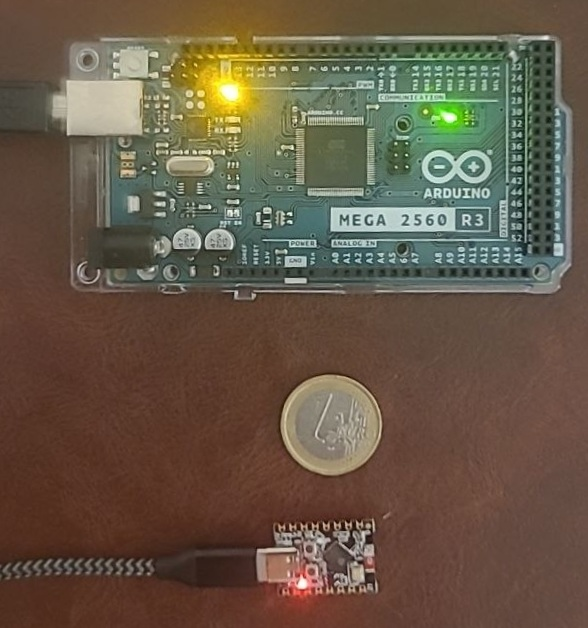
\includegraphics[width=1.95in]{mcu_boards.jpg}
\caption{Physical boards used in the experiments: Arduino Mega 2560 R3 (top) and ESP32-C3 (bottom). The one-euro coin provides a visual size reference only.}
\label{fig:mcu_boards}
\end{figure}

\subsection{Original five-implementation latency and replay consistency}
\begin{table}[t]
\caption{Original five-implementation protocol: measured latency in $\mu$s, mean of five 500-flow pass means and sample SD across those five means. Mega pass means were identical.}
\label{tab:latency}
\centering\footnotesize
\begin{tabular}{lrr}
\toprule
Implementation & Mega 2560 & ESP32-C3\\
\midrule
KAN coefficients & $1396.568\pm0$ & $5.474\pm0.113$\\
KAN sampled LUT & $243.040\pm0$ & $5.889\pm0.201$\\
Multilayer KAN & $12306.176\pm0$ & $55.351\pm0.257$\\
MLP16 & $1328.672\pm0$ & $19.180\pm0.142$\\
DT5 & $17.400\pm0$ & $1.420\pm0.269$\\
\bottomrule
\end{tabular}
\end{table}

\begin{figure*}[!tp]
\centering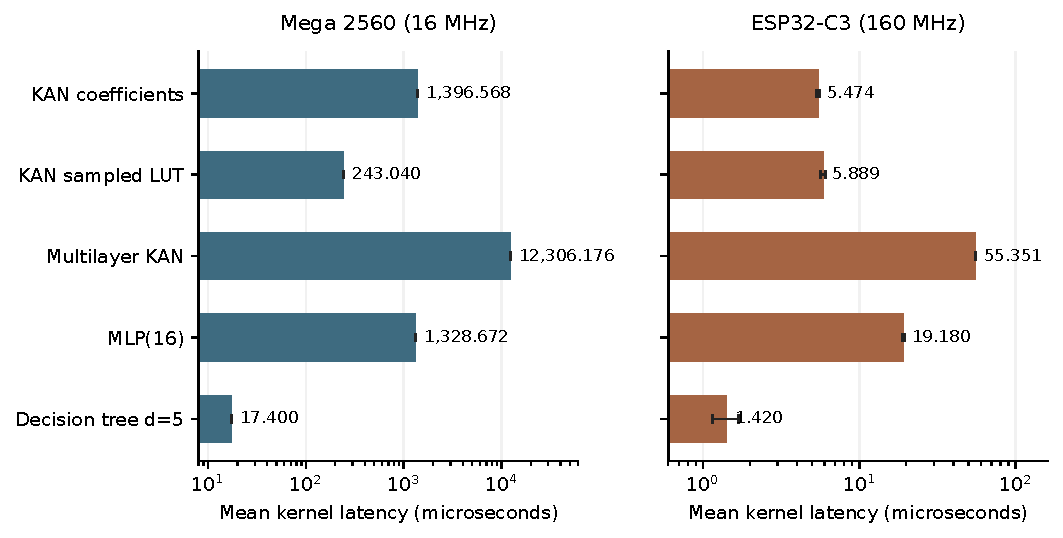
\includegraphics[width=\textwidth]{hardware_latency.pdf}
\caption{Physical inference-kernel latency for the same 500 source flows per pass. Horizontal positions use a logarithmic latency scale; error bars show the sample SD of five reset-separated pass means. Board clocks, framework, and instruction sets differ. Zero observed Mega repeat variation does not imply zero measurement uncertainty.}
\label{fig:latency}
\end{figure*}

Table~\ref{tab:latency} and Fig.~\ref{fig:latency} show a representation trade-off that depends on the processor under the original five-implementation protocol. On the Mega, the LUT reduces mean latency by a factor of 5.746 relative to the coefficient KAN. On the ESP32-C3, its mean is 5.8888~$\mu$s, compared with 5.4740~$\mu$s for coefficients: a 0.4148~$\mu$s increase, or 7.58\%, rather than an observed gain. The experiment does not isolate cache, USB, or instruction-level mechanisms, so no specific causal explanation is assigned to this difference.

DT5 has the smallest observed mean on both targets. Multilayer KAN costs substantially more time than the additive representations, particularly on AVR. These observations concern the fixed implementations and do not rank architectures independently of representation, predictive behavior, or preprocessing.

There are 25 captures and 12,500 measured decisions per board. All 25,000 decisions agree with their compiled C references, and all 12,500 corresponding predictions agree between boards. This is replay consistency, not perfect classification. On the 500 distinct source flows, coefficient KAN, LUT KAN, multilayer KAN, MLP16, and DT5 make 18, 18, 6, 6, and 9 classification errors, respectively. The two additive representations agree on every cohort decision. These cohort counts are not substitutes for the full held-out test metrics.

Individual times lie on a 4-$\mu$s grid on Mega and a 1-$\mu$s grid on ESP32-C3. Raw durations are reported without subtracting timer overhead. The Mega empty probes generally span 0--4~$\mu$s, with 0--8~$\mu$s in the multilayer capture; ESP probes span 0--2~$\mu$s. This matters particularly for the very short DT5 kernel. Identical Mega timing sequences across repeats produce zero sample SD but do not imply zero timing uncertainty. ESP sequences are distinct. There is one board of each type and a fixed implementation order; the SD measures repeat variation on those boards, not manufacturing variation or independent workloads.

\subsection{Separate ESP32-C3 memory-placement diagnostic}
\label{sec:c3diagnostic}
We then tested whether memory placement and repeated-input locality affect the representation trade-off on the same ESP32-C3. This separate experiment retains the frozen weights, $L=1025$, and the same 500 source flows. One application contains two parameter-pointer kernels, one for coefficients and one for the LUT. Each kernel is reused unchanged with its parameters in Flash or copied to DRAM, giving four conditions. The kernels and timing wrappers reside in IRAM; compilation retains \texttt{-Os}, with link-time optimization disabled. ELF sections and reported addresses verify these placements. This application uses 20,808 additional bytes of DRAM parameter payload for the two copies, plus measurement buffers and descriptors; this is not a peak-SRAM measurement.

Five ordered passes run within one boot. Before each of ten collection blocks, 2,000 warm-up calls cover all 500 flows in all four conditions. A four-condition Williams order balances positions and pair precedence over the cohort. Serial operations are absent from warm-up through the end of each collection block, and interrupts remain enabled. The CPU cycle counter measures either one full integer-logit call (\texttt{stream}) or 32 calls on the same input (\texttt{same32}). The latter interval includes the loop and 32 result stores; division by 32 gives an amortized cost, not an isolated-call latency. Timer overhead is not subtracted. At the verified 160-MHz clock, cycles divided by 160 give microseconds. The timing endpoint is the returned integer logit; the binary threshold used by the original protocol is excluded.

\begin{table}[t]
\caption{Separate ESP32-C3 diagnostic in cycles per call: mean and sample SD of five pass means within one boot. The \texttt{same32} column is the amortized 32-call block cost, including the loop and result stores.}
\label{tab:c3diagnostic}
\centering\footnotesize
\begin{tabular}{lrr}
\toprule
Parameters & \texttt{stream} & \texttt{same32}\\
\midrule
Coefficients, Flash & $881.41\pm5.96$ & $832.51\pm0.34$\\
LUT, Flash & $771.80\pm9.15$ & $501.41\pm0.29$\\
Coefficients, DRAM & $820.24\pm1.93$ & $830.39\pm0.26$\\
LUT, DRAM & $482.52\pm1.61$ & $492.96\pm0.43$\\
\bottomrule
\end{tabular}
\end{table}

Within this diagnostic, the LUT reduces the mean \texttt{stream} cost by factors of 1.142 in Flash and 1.700 in DRAM (Table~\ref{tab:c3diagnostic}). The mean gain does not extend to every latency statistic: the pooled \texttt{stream} 95th percentile over 2,500 calls, calculated by linear interpolation and rounded to whole cycles, is 1,482 for the Flash LUT versus 1,119 for Flash coefficients. Moving the parameters from Flash to DRAM reduces this mean by 37.48\% for the LUT and 6.94\% for coefficients. For the LUT, the Flash--DRAM difference is 289.28 cycles per call in \texttt{stream}, but 8.45 amortized cycles per call in \texttt{same32}. Memory access and input locality therefore materially affect the observed cost, and an ESP32-C3 LUT speedup is possible. No cache-miss counter was recorded. These observations do not identify a unique cause of the original 7.58\% increase: code placement, parameter access, timer, timing endpoint, and serial protocol also changed between experiments. The original measurements remain a separate result.

The diagnostic archive contains 20,000 rows representing 330,000 timed calls. Firmware checks found no full-logit mismatches against the frozen, representation-specific references. Single-call logits are transmitted individually; each 32-call row reports the last logit, a checksum, and a mismatch count after all 32 results have been checked outside the timer. These checks establish agreement of the executed diagnostic kernels with their references; five passes within one boot do not constitute independent board or boot replicates.

\section{Retained Twenty-Input USB Pilot}
\label{app:energy-details}
\subsection{Whole-board USB-energy pilot}
\label{sec:energy-pilots}
A separate campaign on 15 September 2026 used an FNIRSI FNB58 USB meter (serial 104332) with the same Mega and ESP32-C3 boards. Five frozen implementations were each evaluated twice on each board, giving twenty physical acquisitions. Figure~\ref{fig:energy-setup} shows the instrumented setups. The meter measures the USB supply to the board and downstream cable; background board consumption is included. The recorded USB identity links the ESP32-C3 series to the earlier board. The photographs illustrate the connections; their screen readings are not used as experimental averages.

\begin{figure*}[t]
\centering
\begin{minipage}[b]{0.47\textwidth}
\centering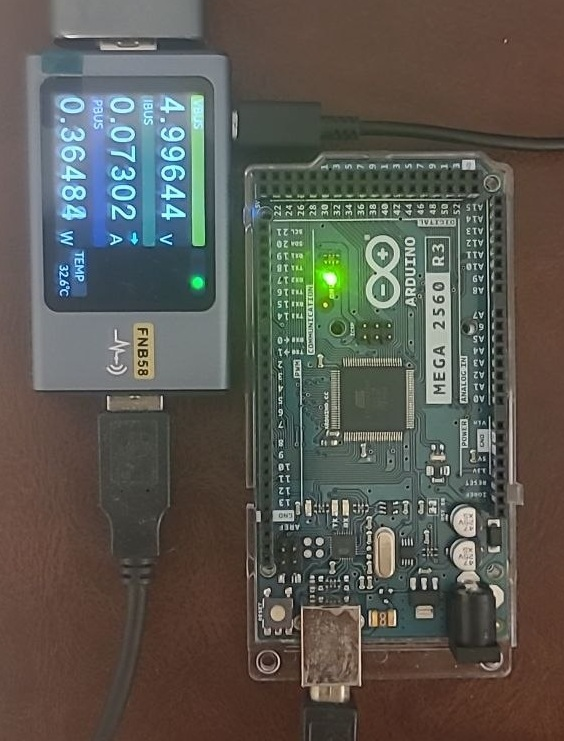
\includegraphics[height=5cm]{Mega_measurement.jpg}\\[-1pt]
{\small (a) Arduino Mega 2560}
\end{minipage}\hfill
\begin{minipage}[b]{0.47\textwidth}
\centering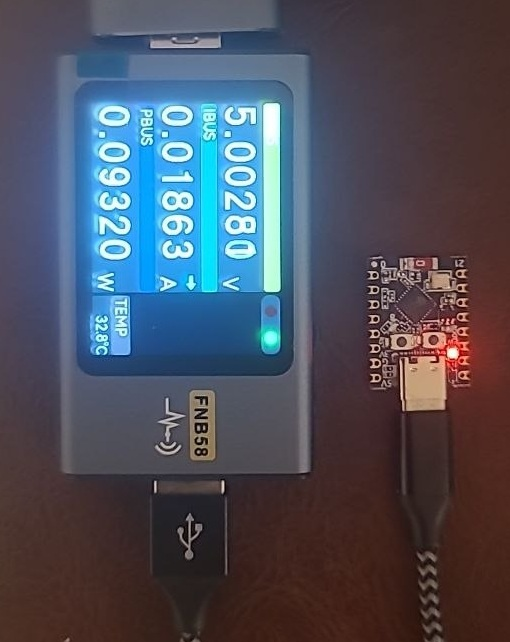
\includegraphics[height=5cm]{C3_measurement.jpg}\\[-1pt]
{\small (b) ESP32-C3}
\end{minipage}
\caption{USB measurement setups for (a) Mega 2560 and (b) ESP32-C3. Displayed voltage, current and power are instantaneous connection snapshots; the results in Table~\ref{tab:energy-pilots} use the archived active-window records. The photographs illustrate the connections, without identifying a particular acquisition.}
\label{fig:energy-setup}
\end{figure*}

Each acquisition repeatedly cycles twenty common source-flow identifiers, using each model's own frozen prepared inputs in RAM. Millions of calls therefore do not represent millions of distinct flows. After warmup, calibration selects a multiple of twenty calls targeting approximately 120 seconds of active execution. The active interval includes the inference call, loop, input indexing, checksum updates and enabled interrupts. Preprocessing, serial output and LED markers are outside this interval. This amortized batch boundary differs from the individual-call boundary in Table~\ref{tab:latency}. On ESP32-C3, the CPU remains at 160~MHz, Wi-Fi and Bluetooth are not initialized, and the active loop contains no explicit yield. The logged watchdog state required no subscription removal in these runs. Frozen parameters remain in Flash; the pilot does not reproduce the DRAM-copy configuration of Table~\ref{tab:c3_followup}.

Power records have a stored spacing of 0.1 seconds. Two LED codes, each with 2-, 4- and 2-second pulses, bracket the active batch. For each record separately, their twelve transition centers define an affine mapping between MCU and meter timestamps. We use the prespecified central 60 seconds of the batch on the MCU clock, mapped to meter times $t_0,t_1$. With linearly interpolated boundary samples and trapezoidal integration of the recorded voltage--current products, the estimator is
\begin{equation}
\overline P=\frac{1}{t_1-t_0}\int_{t_0}^{t_1}V(t)I(t)\,dt,
\qquad
\widehat E_{\rm call}=\overline P\frac{T_{\rm MCU}}{N},
\label{eq:energy-estimator}
\end{equation}
where $T_{\rm MCU}$ is the measured complete active-batch duration and $N$ its call count. This estimates whole-board energy from a stationary central window; it is not the exact integral of the complete active interval or a meter-resolved measurement of an individual call. Idle power is not subtracted. The stored PBUS channel agrees with $VI$. The NRG increment is approximately one quarter of the independently integrated $VI$ total, so that channel is retained for diagnosis and excluded from the estimator without a corrective multiplier.

\begin{table*}[t]
\caption{Separate USB-energy pilot: equal-weight means of two acquisitions per implementation and board. Time is complete active-batch duration divided by call count; power is the central-window USB mean; energy uses~\eqref{eq:energy-estimator}. Each acquisition repeatedly cycles twenty prepared inputs. These descriptive means are not pooled with the 500-flow kernel or placement experiments; displayed digits support reproducibility rather than a stated measurement uncertainty.}
\label{tab:energy-pilots}
\centering\small\setlength{\tabcolsep}{5pt}
\begin{tabular}{lrrrrrr}
\toprule
& \multicolumn{3}{c}{Mega 2560, 16 MHz} & \multicolumn{3}{c}{ESP32-C3, 160 MHz}\\
\cmidrule(lr){2-4}\cmidrule(lr){5-7}
Implementation & Time ($\mu$s) & Power (mW) & Energy ($\mu$J) & Time ($\mu$s) & Power (mW) & Energy ($\mu$J)\\
\midrule
KAN coefficients & 1395.188 & 353.09 & 492.6227 & 5.2133 & 167.78 & 0.8747\\
KAN sampled LUT & 224.842 & 354.19 & 79.6365 & 3.3268 & 165.79 & 0.5516\\
Multilayer KAN & 12223.856 & 355.20 & 4341.9740 & 54.1865 & 173.87 & 9.4216\\
MLP16 & 1340.680 & 356.01 & 477.2986 & 19.8211 & 169.83 & 3.3662\\
DT5 & 15.733 & 358.05 & 5.6332 & 0.7386 & 168.81 & 0.1247\\
\bottomrule
\end{tabular}
\end{table*}

\begin{figure*}[t]
\centering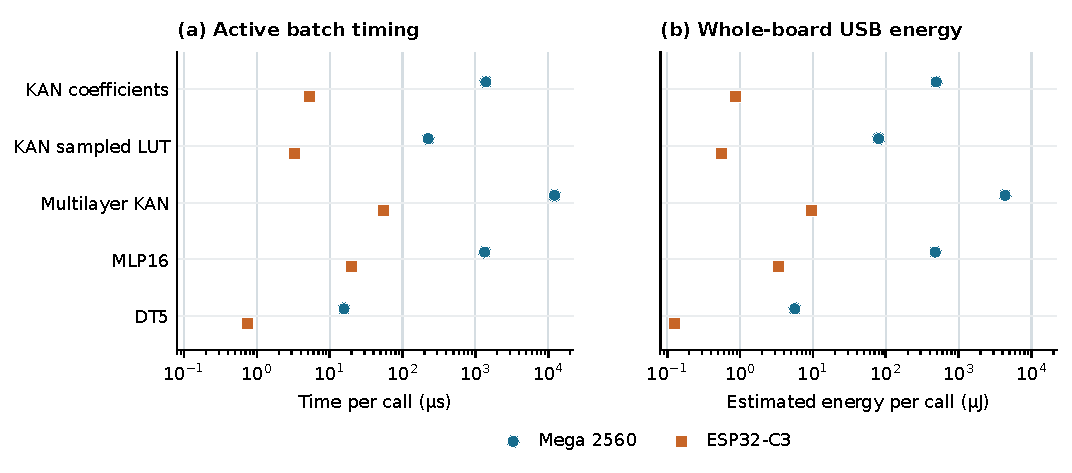
\includegraphics[width=\textwidth]{energy_pilot_comparison.pdf}
\caption{Separate sustained-batch pilot on both boards: amortized time and estimated whole-board energy per call on logarithmic scales. Symbols show the equal-weight mean of two acquisitions, without inferential confidence intervals. The inputs are prepared offline. Processor clocks, toolchains and runtime systems differ, so cross-board ratios do not isolate an instruction-set effect.}
\label{fig:energy-pilots}
\end{figure*}

Table~\ref{tab:energy-pilots} and Fig.~\ref{fig:energy-pilots} show lower LUT cost than coefficient cost within this repeated-input protocol. The LUT reduces amortized time by 83.88\% on Mega and 36.19\% on ESP32-C3; the corresponding energy reductions are 83.83\% and 36.94\%. Similar sustained powers for the two representations make the shorter duration the main contributor to these energy reductions. DT5 has the lowest observed cost, without establishing equal predictive quality. These measurements do not identify the cause of the earlier ESP32-C3 protocol discrepancy.

The implementation order was fixed. The two ESP32-C3 acquisitions of each model share one boot and are separately armed and calibrated. The two energy estimates per model differ by less than 0.32\% on Mega and 0.09\% on ESP32-C3; on ESP32-C3, shifting the central window by $\pm2$ seconds changes its mean power by at most 0.0151\%. These are checks of repeatability and window sensitivity, not instrument accuracy. The visible response spans approximately one second, so the 0.1-second storage grid does not establish a 10-Hz measurement bandwidth. Neither the meter nor the MCU clocks were independently calibrated, and a constant measurement-path delay is not identified by the marker alignment alone. We therefore provide descriptive pilot estimates without an absolute uncertainty budget or confidence intervals formed from correlated power samples.

\begin{table*}[t]
\caption{Energy-pilot application sizes in bytes, separate from the original applications in Table~\ref{tab:memory}. Program use is the linked Flash-use summary; BIN is the actual ESP32-C3 application file length. Static data excludes IRAM, stack and heap peaks.}
\label{tab:pilot-memory}
\centering\small\setlength{\tabcolsep}{5pt}
\begin{tabular}{lrrrrr}
\toprule
& \multicolumn{2}{c}{Mega 2560} & \multicolumn{3}{c}{ESP32-C3}\\
\cmidrule(lr){2-3}\cmidrule(lr){4-6}
Implementation & Program use & Static data & Program use & Data/BSS & BIN\\
\midrule
KAN coefficients & 22,300 & 841 & 267,790 & 15,888 & 283,856\\
KAN sampled LUT & 42,060 & 841 & 287,962 & 15,888 & 300,016\\
Multilayer KAN & 28,266 & 841 & 273,118 & 15,904 & 285,248\\
MLP16 & 22,310 & 841 & 268,144 & 15,888 & 283,728\\
DT5 & 23,232 & 917 & 269,486 & 15,968 & 283,520\\
\bottomrule
\end{tabular}
\end{table*}

The source, upload and run records agree with the delivered frozen headers. Inspection of all five actual ESP32-C3 ELF files confirms that a real inference call remains inside the measured count-controlled loop and is followed by checksum accumulation. Model constants match the frozen source, and the application BIN segments agree with the corresponding ELF sections. Prepared-input decisions matched the compiled references, and active-batch checksums matched their expected sums; the checksum does not verify every active decision separately. These checks support the execution and provenance claims; they do not make this small repeated workload a detection-quality evaluation.


The following table preserves the original pilot means for audit against the full-precision CSV. The pilot remains separate from the HW500 study; these digits imply no absolute instrument accuracy.
\begin{table*}[p]
\caption{Full retained numerical precision for the separate USB-energy pilot: equal-weight means of two acquisitions per implementation and board. Time is complete active-batch duration divided by call count; power is the central-window USB mean; energy uses~\eqref{eq:energy-estimator}. Each acquisition repeatedly cycles twenty prepared inputs. These descriptive means are not pooled with the 500-flow kernel or placement experiments; displayed digits support reproducibility rather than a stated measurement uncertainty.}
\label{tab:energy-pilots-full}
\centering\small\setlength{\tabcolsep}{5pt}
\begin{tabular}{lrrrrrr}
\toprule
& \multicolumn{3}{c}{Mega 2560, 16 MHz} & \multicolumn{3}{c}{ESP32-C3, 160 MHz}\\
\cmidrule(lr){2-4}\cmidrule(lr){5-7}
Implementation & Time ($\mu$s) & Power (mW) & Energy ($\mu$J) & Time ($\mu$s) & Power (mW) & Energy ($\mu$J)\\
\midrule
KAN coefficients & 1395.188 & 353.09 & 492.6227 & 5.2133 & 167.78 & 0.8747\\
KAN sampled LUT & 224.842 & 354.19 & 79.6365 & 3.3268 & 165.79 & 0.5516\\
Multilayer KAN & 12223.856 & 355.20 & 4341.9740 & 54.1865 & 173.87 & 9.4216\\
MLP16 & 1340.680 & 356.01 & 477.2986 & 19.8211 & 169.83 & 3.3662\\
DT5 & 15.733 & 358.05 & 5.6332 & 0.7386 & 168.81 & 0.1247\\
\bottomrule
\end{tabular}
\end{table*}


\section{Additional Classification Results}
\label{app:results}
The following tables retain native binary and multiclass summaries, both class recalls for the rich joint-source experiments, and the validation ratio criterion. Their standard deviations describe the recorded repeat units, as stated in each caption. The supplied run-level CSVs retain additional metrics and full numerical precision. No model fitting was repeated when these summaries were checked.
% Supplementary ML tables. Requires \usepackage{booktabs}.
% ML values are author-saved. Mean/sample-SD consistency was independently
% recomputed from saved run CSVs; no models were refitted for this draft.

\begin{table*}[t]
\centering
\caption{Joint-model results in the rich harmonized space. Values are means $\pm$ sample SD on the 0--1 scale across ten fits (seeds 42--51). Final fitting uses 4,584 equally contributed source observations. Normal recall equals $1-\mathrm{FPR}$. Test-population sizes and source balancing are specified in the methods.}
\label{tab:supp-joint-recalls}
\footnotesize
\setlength{\tabcolsep}{6pt}
\begin{tabular}{llccc}
\toprule
Evaluation domain & Model & Balanced accuracy & Normal recall & Attack recall \\
\midrule
TON\_IoT & Additive KAN & $0.9432 \pm 0.0016$ & $0.9558 \pm 0.0029$ & $0.9306 \pm 0.0032$ \\
 & Multilayer KAN & $0.9811 \pm 0.0014$ & $0.9706 \pm 0.0035$ & $0.9916 \pm 0.0015$ \\
 & MLP16 & $0.9296 \pm 0.0083$ & $0.8720 \pm 0.0236$ & $0.9872 \pm 0.0078$ \\
 & DT5 & $0.9669 \pm 0.0056$ & $0.9512 \pm 0.0108$ & $0.9827 \pm 0.0108$ \\
 & LightGBM & $0.9846 \pm 0.0017$ & $0.9751 \pm 0.0039$ & $0.9941 \pm 0.0014$ \\
 & XGBoost & $0.9804 \pm 0.0030$ & $0.9673 \pm 0.0072$ & $0.9935 \pm 0.0016$ \\
\midrule
BoT-IoT & Additive KAN & $0.9825 \pm 0.0110$ & $0.9705 \pm 0.0226$ & $0.9944 \pm 0.0011$ \\
 & Multilayer KAN & $0.9924 \pm 0.0057$ & $0.9884 \pm 0.0116$ & $0.9964 \pm 0.0004$ \\
 & MLP16 & $0.9494 \pm 0.0166$ & $0.9032 \pm 0.0332$ & $0.9956 \pm 0.0006$ \\
 & DT5 & $0.9865 \pm 0.0094$ & $0.9768 \pm 0.0184$ & $0.9962 \pm 0.0007$ \\
 & LightGBM & $0.9951 \pm 0.0027$ & $0.9937 \pm 0.0054$ & $0.9964 \pm 0.0002$ \\
 & XGBoost & $0.9925 \pm 0.0044$ & $0.9884 \pm 0.0092$ & $0.9966 \pm 0.0007$ \\
\midrule
UNSW-NB15 & Additive KAN & $0.3991 \pm 0.0228$ & $0.5125 \pm 0.0451$ & $0.2857 \pm 0.0089$ \\
 & Multilayer KAN & $0.3629 \pm 0.0614$ & $0.3394 \pm 0.1070$ & $0.3865 \pm 0.1197$ \\
 & MLP16 & $0.3119 \pm 0.0094$ & $0.2783 \pm 0.0182$ & $0.3454 \pm 0.0051$ \\
 & DT5 & $0.4081 \pm 0.0619$ & $0.4707 \pm 0.0945$ & $0.3456 \pm 0.1031$ \\
 & LightGBM & $0.3884 \pm 0.0793$ & $0.3723 \pm 0.1101$ & $0.4044 \pm 0.1814$ \\
 & XGBoost & $0.4193 \pm 0.0428$ & $0.4264 \pm 0.0869$ & $0.4121 \pm 0.1030$ \\
\bottomrule
\end{tabular}
\end{table*}

% Source: work/results/cv_leakagefree_summary_binary_ALL.csv and
% work/results/cv_leakagefree_summary_multiclass_ALL.csv.
\begin{table*}[t]
\centering
\caption{Native TON\_IoT cross-validation. Values are means $\pm$ sample SD on the 0--1 scale across 15 fits: five folds for seeds 42--44, stratified by the ten-class label. Feature selection and preprocessing use each training fold. These floating-point results are separate from canonical integer deployment.}
\label{tab:supp-native-cv}
\footnotesize
\setlength{\tabcolsep}{6pt}
\begin{tabular}{lcccc}
\toprule
& \multicolumn{2}{c}{Binary classification} & \multicolumn{2}{c}{Ten-class classification} \\
\cmidrule(lr){2-3}\cmidrule(lr){4-5}
Model & Balanced accuracy & Attack F1 & Balanced accuracy & Macro-F1 \\
\midrule
Additive KAN & $0.9765 \pm 0.0009$ & $0.9835 \pm 0.0007$ & $0.9295 \pm 0.0023$ & $0.8767 \pm 0.0014$ \\
Multilayer KAN & $0.9963 \pm 0.0004$ & $0.9976 \pm 0.0002$ & $0.9738 \pm 0.0019$ & $0.9374 \pm 0.0036$ \\
MLP16 & $0.9934 \pm 0.0014$ & $0.9964 \pm 0.0009$ & $0.9151 \pm 0.0154$ & $0.9182 \pm 0.0107$ \\
DT5 & $0.9919 \pm 0.0007$ & $0.9944 \pm 0.0004$ & $0.7864 \pm 0.0037$ & $0.7633 \pm 0.0033$ \\
LightGBM & $0.9983 \pm 0.0003$ & $0.9991 \pm 0.0001$ & $0.9807 \pm 0.0020$ & $0.9680 \pm 0.0021$ \\
XGBoost & $0.9975 \pm 0.0004$ & $0.9989 \pm 0.0001$ & $0.9737 \pm 0.0028$ & $0.9666 \pm 0.0021$ \\
\bottomrule
\end{tabular}
\end{table*}

% Source: work/results/joint_ratio_selection_runs.csv.
% Aggregation unit: first mean across 6 models x 2 domains within seed,
% then mean and sample SD across ten seeds; not SD across 120 mixed cells.
\begin{table*}[t]
\centering
\caption{Validation ratio selection, on the 0--1 balanced-accuracy scale. Each seed first averages six models and two validation domains; reported SD is across ten seed means. Counts refer to inner training fits, not final refitting. The corrected criterion does not undo historical test-set inspection.}
\label{tab:supp-ratio-selection}
\footnotesize
\setlength{\tabcolsep}{6pt}
\begin{tabular}{ccrrr}
\toprule
Normal:attack & Validation balanced accuracy & Normal/domain & Attack/domain & Union fit rows \\
\midrule
$1:5$ & $0.9732 \pm 0.0041$ & 306 & 1530 & 3672 \\
$1:10$ & $0.9702 \pm 0.0049$ & 306 & 3060 & 6732 \\
$1:20$ & $0.9657 \pm 0.0064$ & 306 & 6120 & 12852 \\
$1:50$ & $0.9592 \pm 0.0060$ & 306 & 15300 & 31212 \\
$1:100$ & $0.9523 \pm 0.0042$ & 306 & 30600 & 61812 \\
\bottomrule
\end{tabular}
\end{table*}

% Source: work/results/crossdomain_summary_cat.csv; sample SD checked
% against work/results/crossdomain_runs_cat.csv.
\begin{table*}[t]
\centering
\caption{Rich-space single-source balanced accuracy, mean $\pm$ sample SD on the 0--1 scale. In-domain columns summarize 50 fits; transfer columns summarize ten fits (seeds 42--51). The 50:1 attack:normal cap affects training only. Tests retain natural priors; repeat variability does not represent independent networks.}
\label{tab:supp-cross-dispersion}
\footnotesize
\setlength{\tabcolsep}{6pt}
\begin{tabular}{lcccc}
\toprule
Model & TON$\to$TON & BoT$\to$BoT & TON$\to$BoT & BoT$\to$TON \\
\midrule
Additive KAN & $0.9701 \pm 0.0012$ & $0.9934 \pm 0.0010$ & $0.5573 \pm 0.0095$ & $0.6112 \pm 0.0695$ \\
Multilayer KAN & $0.9932 \pm 0.0007$ & $0.9971 \pm 0.0027$ & $0.4588 \pm 0.0548$ & $0.6855 \pm 0.0977$ \\
MLP16 & $0.9879 \pm 0.0016$ & $0.9426 \pm 0.0361$ & $0.4369 \pm 0.0634$ & $0.7343 \pm 0.0144$ \\
DT5 & $0.9828 \pm 0.0015$ & $0.9952 \pm 0.0034$ & $0.5494 \pm 0.0089$ & $0.4597 \pm 0.0107$ \\
LightGBM & $0.9963 \pm 0.0004$ & $0.9971 \pm 0.0031$ & $0.4779 \pm 0.0083$ & $0.6964 \pm 0.0545$ \\
XGBoost & $0.9947 \pm 0.0004$ & $0.9779 \pm 0.0087$ & $0.5528 \pm 0.0269$ & $0.6487 \pm 0.0461$ \\
\bottomrule
\end{tabular}
\end{table*}


\raggedbottom
\section{Descriptive Factorial Contrasts}
\label{app:factorial}
For each of the eight passes, let $y_{abc}$ be the mean latency of its 500 calls under condition $(a,b,c)\in\{-1,1\}^3$. For a nonempty factor set $S$, the reported contrast is $e_S=\frac14\sum_{a,b,c}(\prod_{j\in S}x_j)y_{abc}$. Main contrasts average over the other factors; two-factor contrasts are half a difference-in-differences. Table~\ref{tab:c3-factorial} reports the mean and sample SD of the eight paired pass contrasts. The passes reuse one device and a fixed cohort; no population-level ANOVA significance or independence of individual calls is assumed.
\begin{table}[t]
\centering
\caption{Descriptive factorial contrasts of the eight ESP32-C3 pass means. $A$: LUT minus coefficients; $B$: IRAM minus Flash code; $C$: DRAM minus Flash parameters. A two-factor contrast is half a difference-in-differences, and the three-factor contrast is one quarter of the triple difference. SD is across the eight paired pass contrasts on one board. Negative values indicate a lower mean latency for the positive contrast.}
\label{tab:c3-factorial}
\begin{tabular}{lrr}
\toprule
Contrast & Effect ($\mu$s) & Pass SD ($\mu$s)\\
\midrule
$A$ & -1.9016 & 0.0040\\
$B$ & -0.0694 & 0.0060\\
$C$ & -0.2290 & 0.0038\\
$AB$ & -0.0573 & 0.0046\\
$AC$ & -0.2168 & 0.0040\\
$BC$ & 0.0853 & 0.0044\\
$ABC$ & 0.0649 & 0.0043\\
\bottomrule
\end{tabular}
\end{table}


\section{Source-to-Cache and Source--Target Checks}
\label{app:data-checks}
The retained source sampler was reconstructed for seeds 42--51 without model fitting. Twenty domain-specific index selections agree with the retained sampling function, and their sizes agree with the saved run records: 382 normal and 1,910 attack observations per domain, or 4,584 combined rows. This reconstruction is conditional on the supplied caches, retained code and the verification environment (scikit-learn 1.8.0); historical index hashes and fitted objects are unavailable. It does not establish bit-identical replay of the original training runs.

\begin{table}[t]
\caption{Category associations in reconstructed balanced joint cohorts ($J$) and UNSW ($U$). $P_D=P_D(attack\mid c)$ and $LR_D=P_D(c\mid attack)/P_D(c\mid normal)$. Joint intervals are minima--maxima over ten reconstructed cohorts, not confidence intervals.}
\label{tab:unsw-category-shift}
\centering\scriptsize\setlength{\tabcolsep}{2.4pt}
\begin{tabular}{lrrrr}
\toprule
Category $c$ & $P_J$ & $P_U$ & $LR_J$ & $LR_U$\\
\midrule
\multicolumn{5}{l}{Protocol}\\
\texttt{other} & 0.0000 & 0.9046 & 0.000 & 5.358\\
\texttt{tcp} & 0.9334--0.9445 & 0.4557 & 2.803--3.406 & 0.473\\
\texttt{udp} & 0.6738--0.6866 & 0.7625 & 0.413--0.438 & 1.813\\
\midrule
\multicolumn{5}{l}{State}\\
\texttt{closed} & 0.8884--0.9105 & 0.4764 & 1.591--2.034 & 0.514\\
\texttt{established} & 0.4487--0.4892 & 0.0697 & 0.163--0.192 & 0.042\\
\bottomrule
\end{tabular}
\end{table}

The full \texttt{other} category comprises 41,916 UNSW rows. Of these, 37,760 reach it through the protocol fallback; 4,156 ARP rows use an explicit mapping. The zero unseen-category rate therefore does not mean that the original protocol composition is unchanged. Normalizing category frequencies within each class through $LR$ separates these associations from the overall attack proportion. An $LR$ above one favors occurrence among attacks; it is not a learned model parameter.

Nine of thirteen candidate numerical features have opposite marginal Spearman signs between every reconstructed joint cohort and UNSW; seven also have $|\rho|>0.05$ on both sides for every seed. Such counts do not establish independent mechanisms. The saved MI selections exclude \texttt{pkts\_dst} and \texttt{payload\_mean\_dst} in every joint seed, while \texttt{bytes\_dst} is selected in eight. In the common TCP/\texttt{closed} stratum, destination-feature correlations are negative in both full TON and UNSW. Thus a full-population sign reversal need not survive conditioning or source balancing.

Zero duration creates large rate values through the fixed $10^{-6}$ denominator offset. Nevertheless, zero duration is relatively associated with normal traffic in both the reconstructed joint mixture and UNSW. The target subset contains 3,543 normal and 64 attack rows. Correcting all errors exclusively on that subset could increase BA by at most $\tfrac12(3543/93000+64/164673)=0.019243$, or 1.9243 percentage points. This cannot account for the entire observed deficit to 0.5; it does not rule out broader effects of rate features during learning. No denominator or mapping was retuned on the target.

The checks also reproduce all sixteen TON cache columns from 211,043 source rows and verify binary labels against attack types. For UNSW, source-file identity and row position are retained together because the raw \texttt{id} values repeat across training and testing CSVs. Exact transformation agreement establishes numerical consistency of this segment, not semantic equivalence of different flow extractors or correctness of the subsequent unavailable fitted-model path. The detailed outputs distinguish the smoothed ratios $b/(p+1)$ from physical bytes per packet and report the actual size of percentile-threshold subsets when tied values exceed one percent.

The six recovered JSONL checkpoint files contain 900 model--seed--domain evaluation records, including the 420 current rich/reduced records and 480 from the superseded ratio grid. Their values agree with the saved run tables, and confusion-derived metrics and aggregate means and sample standard deviations were independently recomputed. Twelve pooled matrices in the superseded ratio-50 grid omit seed 42; the original matrices are retained with separate corrected sums. These archival corrections do not alter the current validation-only selection or the per-fit means reported in this article. The checkpoints contain aggregates, not the predictions needed to reconstruct ROC/PR curves or attribute individual UNSW errors.


\section*{Acknowledgment}
ChatGPT (OpenAI) assisted with drafting and editing throughout the manuscript and with supporting code, under human supervision. The authors retain responsibility for the methods, results, and final content.

\bibliographystyle{IEEEtran}
\bibliography{references}

\noindent\begin{minipage}{\columnwidth}
\phantomsection
\begin{IEEEbiography}[{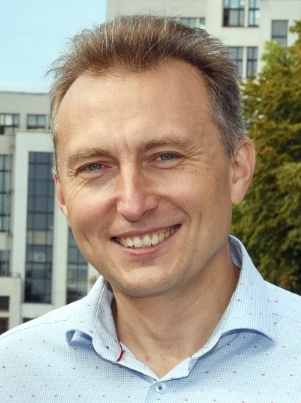
\includegraphics[width=1in,height=1.25in,clip,keepaspectratio]{figures/Kuznetsov.png}}]{Oleksandr Kuznetsov}
(Member, IEEE) is an Associate Professor at the Department of Theoretical and Applied Sciences, eCampus University, Italy, and a Full Professor at the Department of Intelligent Software Systems and Technologies, V.N. Karazin Kharkiv National University, Ukraine. He holds a Doctor of Sciences degree and is a laureate of the Boris Paton National Prize of Ukraine (2021), the nation's highest academic distinction, in recognition of his contributions to cybersecurity and cryptographic information protection systems. His career spans over two decades, with leadership roles across academia, industry, and defense. He served as a Senior Data Scientist at Proxima Labs, San Francisco, from 2023 to 2024, developing trustless computation platforms using zero-knowledge proofs, and as Chief Scientist at Grape Blockchain, London, from 2022 to 2023, working on DAG-based consensus mechanisms. His research interests include applied cryptography, post-quantum security, blockchain and decentralized systems, artificial intelligence in cybersecurity, biometric authentication, steganography, and IoT security.
\end{IEEEbiography}
\end{minipage}\par

\newpage
\noindent\begin{minipage}{\columnwidth}
\phantomsection
\begin{IEEEbiography}[{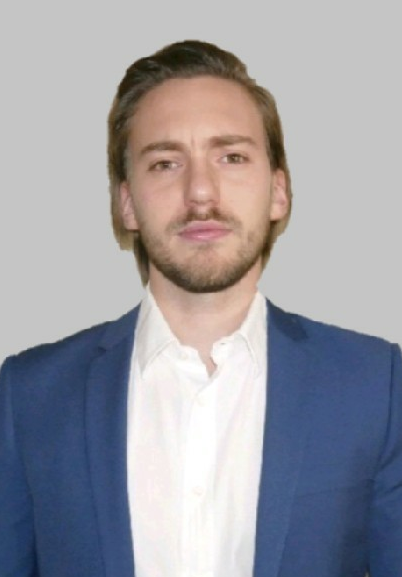
\includegraphics[width=1in,height=1.25in,clip,keepaspectratio]{figures/E_P_Bernardis.png}}]{Emanuele Pio De Bernardis}
has an academic background in Computer and Automation Engineering at eCampus University, Italy. Since 2025, he has been a research collaborator with Oleksandr Kuznetsov at eCampus University, working on machine learning for cybersecurity and deployment on resource-constrained devices. His research interests include edge artificial intelligence, model quantization, intrusion detection for Internet of Things and Industrial Internet of Things networks, and reproducible scientific software. His work covers data preprocessing, feature engineering, supervised model evaluation, integer quantization, and embedded inference pipelines. He also works on feature attribution and the assessment of generalization under distribution shift. His software experience includes Python-based machine learning pipelines, TensorFlow Lite Micro, C-code model export, and version-controlled experimental workflows. He holds the IBM AI Engineering and IBM Data Science Professional Certificates. Before focusing on academic studies and research, he accumulated eleven years of operational and managerial experience, including responsibility for performance monitoring and structured reporting. This background informs his interest in practical, maintainable machine learning systems.
\end{IEEEbiography}
\end{minipage}\par

\noindent\begin{minipage}{\columnwidth}
\phantomsection
\begin{IEEEbiography}[{
\includegraphics[width=1in,height=1.25in,clip,keepaspectratio]{figures/fronto.png}}]{Emanuele Frontoni}
(Member, IEEE) is a Full Professor of computer science with the University of Macerata and the Co-Director of the VRAI Vision Robotics \& Artificial Intelligence Lab. His research interests include computer vision and artificial intelligence, with applications in robotics, video analysis, human behavior analysis, extended reality, and digital humanities. He is the author of over 230 international articles and collaborates with national and international companies in technology transfer and innovation. He has served as a program chair or general chair of international conferences and summer schools, including IEEE/ASME MESA Mechatronic and Embedded Systems and Applications in 2016 and 2017, IEEE ECMR European Conference on Mobile Robotics in 2017, BigDat 2020, and DeepLearn 2021. He has also co-organized international workshops, including DeepRetail at ICPR 2020, D2CH at CVPR 2021, and AI4DH at ICIAP 2022.
\end{IEEEbiography}
\end{minipage}\par
\EOD
\end{document}
